\documentclass{report}

% Language setting
% Replace `english' with e.g. `spanish' to change the document language
\usepackage[english]{babel}

% Set page size and margins
% Replace `letterpaper' with `a4paper' for UK/EU standard size
\usepackage[letterpaper,top=2cm,bottom=2cm,left=3cm,right=3cm,marginparwidth=1.75cm]{geometry}

% Useful packages
\usepackage[colorlinks=true, allcolors=black]{hyperref}
\usepackage{amsmath}
\usepackage{amsthm}
\usepackage{amsfonts}
\usepackage{graphicx}
\usepackage{stmaryrd}
\usepackage{amssymb}
\usepackage{ebproof}
\usepackage{listings}
\usepackage{xcolor}
\usepackage{csquotes}
\usepackage{ulem}
\usepackage{tikz}
\usepackage{mathtools}
%% \usepackage{mathaccents}

\definecolor{codegreen}{rgb}{0,0.6,0}
\definecolor{codegray}{rgb}{0.5,0.5,0.5}
\definecolor{codepurple}{rgb}{0.58,0,0.82}
\definecolor{backcolour}{rgb}{0.97,0.98,0.99}

\usepackage{listings}
\usepackage{courier}
\lstset{
    basicstyle=\footnotesize\ttfamily, % Default font
    % numbers=left,              % Location of line numbers
    numberstyle=\tiny,          % Style of line numbers
    % stepnumber=2,              % Margin between line numbers
    numbersep=5pt,              % Margin between line numbers and text
    tabsize=2,                  % Size of tabs
    extendedchars=true,
    breaklines=true,            % Lines will be wrapped
    keywordstyle=\color{red},
    frame=b,
    % keywordstyle=[1]\textbf,
    % keywordstyle=[2]\textbf,
    % keywordstyle=[3]\textbf,
    % keywordstyle=[4]\textbf,   \sqrt{\sqrt{}}
    stringstyle=\color{white}\ttfamily, % Color of strings
    showspaces=false,
    showtabs=false,
    xleftmargin=17pt,
    framexleftmargin=17pt,
    framexrightmargin=5pt,
    framexbottommargin=4pt,
    backgroundcolor=\color{backcolour},
    showstringspaces=false
}
\lstloadlanguages{ % Check documentation for further languages ...
     % [Visual]Basic,
     % Pascal,
     % C,
     % C++,
     % XML,
     % HTML,
     Haskell,
     Scala,
     Prolog
}
% \DeclareCaptionFont{blue}{\color{blue}} 

% \captionsetup[lstlisting]{singlelinecheck=false, labelfont={blue}, textfont={blue}}
\usepackage{caption}
\DeclareCaptionFont{white}{\color{white}}
\DeclareCaptionFont{black}{\color{black}}
\DeclareCaptionFormat{listing}{\colorbox[rgb]{1,0,0}{\parbox{\textwidth}{\hspace{15pt}#1#2#3}}}
\captionsetup[lstlisting]{format=listing,labelfont=white,textfont=white, singlelinecheck=false, margin=0pt, font={bf,footnotesize}}


\theoremstyle{definition}
\newtheorem{example}{Example}[section]

\theoremstyle{definition}
\newtheorem{definition}{Definition}[section]
\newtheorem*{definition*}{Definition}



% \lstdefinestyle{mystyle}{
%     backgroundcolor=\color{backcolour},   
%     commentstyle=\color{codegreen},
%     keywordstyle=\color{magenta},
%     numberstyle=\tiny\color{codegray},
%     stringstyle=\color{codepurple},
%     basicstyle=\ttfamily\footnotesize,
%     breakatwhitespace=true,         
%     breaklines=true,                 
%     captionpos=b,                    
%     keepspaces=true,                                  
%     showspaces=false,                
%     showstringspaces=false,
%     showtabs=false,                  
%     tabsize=2,
%     framextopmargin=6pt,
%     framexbottommargin=6pt, 
%     frame=tb,
%     framerule=0pt
% }
% \lstset{style=mystyle}

\newcommand{\bhref}[2]{\textbf{\href{#1}{#2}}}
\newcommand{\repo}[1]{\bhref{#1}{[Repository]}}
\newcommand{\ttt}[1]{\texttt{#1}}
\newcommand{\ttb}[1]{\textbf{\ttt{#1}}}
\newcommand{\alt}{\;\; | \;\;}
\newcommand{\tab}{\;\;\;}
\newcommand{\tav}{\;\;}
\newcommand{\hookuparrow}{\mathrel{\rotatebox[origin=c]{90}{$\hookrightarrow$}}}
\newcommand{\hookdownarrow}{\mathrel{\rotatebox[origin=c]{-90}{$\hookrightarrow$}}}
\newcommand{\SLongdownarrow}{\mathrel{\rotatebox[origin=c]{-90}{$\Longrightarrow$}}}
\newcommand{\updownsquigarrow}{\mathrel{\rotatebox[origin=c]{-90}{$\leftrightsquigarrow$}}}
\newcommand\nldots{\stackrel{\mathclap{\normalfont\mbox{n}}}{\ldots}}
\newcommand{\kldots}[1]{\stackrel{\mathclap{\normalfont\mbox{#1}}}{\ldots}}




\title{Type-Based Test Generation for Haskell and Scala using Constraint Logic Programming}
\author{Rafael Fernández Ortiz}

\begin{document}
\maketitle
\begin{abstract}
	Building \textit{generators} to create test cases that Property-Based Testing use to test software behavior is a hard, quite costly, and error-prone task. Even though most Property-Based Testing frameworks cover simple scenarios, there is some kind of issues with preconditioned generated test cases.
	\\\\
	%%
	In the context of Property-Based Testing for strong and statically well-typed languages, such as Haskell or Scala, we propose an approach to relieve the programmer from the task of writing generators.\\\\
	%%
	Our approach consists in provide an efficient and automatic generation of input test values that satisfy a given specification. In particular, we consider the case when the input values are algebraic data types satisfying complex constraints. The generation process is performed by writing specification expressions driven by the language' syntax and via symbolic execution using constraint logic programming.
\end{abstract}
\tableofcontents

\chapter{Introduction}

Software is a set of instructions that tell a computer what to do. It can be used for various tasks, from simple calculations to complex simulations. Confidence in software is important because it ensures that the software will perform as expected and not cause unintended consequences. Unfortunately, that confidence is not present most time.\\\\
Software risks can come from various sources, such as bugs, security vulnerabilities, or poor design. These risks can lead to errors, crashes, or even loss of data.\\\\
For critical systems, such as those used in the medical or aerospace industries, the stakes are even higher. These systems must be thoroughly tested and validated to ensure that they will not cause harm or failure in a critical situation. For example:
\begin{itemize}
	\item Medical systems: Medical systems such as electronic health records (EHRs) and medical devices are critical systems that can have serious consequences if they fail. A bug in an EHR system could lead to incorrect patient information being displayed, potentially leading to a misdiagnosis or other medical errors.
	\item Aerospace systems: Aerospace systems such as aircraft navigation systems and flight control systems are critical systems that must operate reliably at all times. A bug in an aircraft navigation system could cause the plane to fly off course, leading to a crash.
	\item Industrial control systems: Industrial control systems (ICS) are used to control and monitor industrial processes such as manufacturing, power generation, and oil and gas production. An issue in an ICS could cause a malfunction in a manufacturing process, leading to costly downtime or even physical damage to the equipment, or even a cyber-attack on an ICS could cause a shutdown of the whole process causing a major disruption.
\end{itemize}
When we talk about software quality, we are talking about how well a software system or application meets its specified requirements and is fit for its intended use. It is a multi-faceted concept that includes aspects such as whether the software performs the intended tasks, and whether it meets the needs of the end users. That is functionality. Also, it includes other factors such as reliability, usability, performance, and maintainability.\\\\
Ensuring that software has good functionality, or more generally, ensuring software quality is important because it helps to ensure that the software will be useful, effective and that it will perform as expected and not cause unintended consequences. for its intended purpose.\\\\
In order to guarantee the expected behavior and therefore, to have good software quality, testing and validation are critical for identifying and mitigating these issues.
%
\pagebreak
%
\section{Testing}

Software testing (or simply testing) is the process of evaluating a system or its component(s) to find whether it satisfies the specified requirements. It consists of executing a program on a known pre-selected set (test suite) of inputs (test cases) and inspecting whether the outputs match the expected results.\\\\
This process validates the semantic properties of a program's behavior. It's important to test software thoroughly before deployment to ensure it functions as intended and to identify and fix bugs or other issues. Testing is an essential step in the software development process and is critical for ensuring the quality and reliability of software.\\\\
Therefore, we can define in a relaxed way that a \textbf{test} is a set of executions on a given program using different input data for each execution; its purpose is to determine if the program functions correctly. A test has a negative result if an error is detected during the test i.e., the program crashes or \textbf{a property is violated}. \\

A test has a positive result if a series of tests produces no error, and the series of tests is "complete" under some coverage metric. When we say in software testing that a test is "complete", it refers to the level of coverage the tests provide for the software being tested. In other words, that reflects a representative percentage of the reliability of the software with respect to expected behavior. However, we have to consider that "reliability" is relative and it is biased and subject to the chosen test cases, which is itself subject to the criteria of the tester.\\

A test has an "incomplete" result if a series of tests produces no errors but the series is not complete under the coverage metric. In summary, a test is focused on evaluating the software to find any issues and bugs.\\\\
There are different types of tests that can be used during the software development process, each with a different purpose and focus. Some of the main types of tests are:
%%
\begin{itemize}
	\item \textbf{Unit testing}: Unit testing is a type of testing that focuses on individual components of the software, such as individual functions or methods. Unit testing aims to ensure that each component behaves as expected. Unit tests are usually automated, and they are run as part of the development process to catch any issues early.
	\item \textbf{Integration testing}: Integration testing is used to ensure that different software components work together correctly. It tests the interactions between different parts of the software. Integration tests are usually automated, and they are run after the unit tests to ensure that the integrated system behaves as expected.
	\item \textbf{Acceptance testing}: Acceptance testing is used to ensure that the software meets the needs of the end users. It is typically done by the customer or other stakeholders to ensure that the software meets their needs. Acceptance tests can be automated or manual, and they are run after system tests to ensure that the system is ready to be deployed.
\end{itemize}
%%
Sadly, trying to find counter-examples by testing that produces bugs a behavior non-expected is most of the time a difficult task. In simpler software, testers could find most of those cases which produce counter-examples, designing test cases one by one. However, the design process reaches those cases that one knows by experience or intuition, leaving aside very interesting and not at all intuitive cases that can hardly be imagined. For this reason and because it can be a very tedious task, it would be ideal to automate the generation of test cases.

\subsubsection*{Test Driven Development or Correctness by Constructions?}
%% Revisar
Also, during the life-cycle of software development has used several known techniques in order to get free-bugs software in an efficient and proper way. The most common paradigm, which is also the most natural way, is \textbf{Test Driven Development} (a.k.a TDD).\\

TDD is a software development technique in which tests are developed before the code, in short and incremental cycles. This technique proposes for the developer to create a new flawed test, and then to implement a little piece of code, in order to satisfy the current test set. Then, the code is refactored if necessary, to provide a better structure and architecture for the current solution. \\\\
%%
The challenge addressed in this work is to use TDD in applications with non-deterministic behavior as stated before. Although it is not possible to know exactly what the output will be, it is usually possible to check whether the generated output is valid or not.\\\\
%%
The following factors make it difficult to develop randomized software using TDD: 
\begin{itemize}
	\item Results for each execution may be different for the same inputs, which makes it difficult to validate the return value.
	\item Obtaining a valid return for a test case execution does not mean that valid return will be delivered on the next executions.
	\item The random decisions and their paths number make it not viable to create Mock Objects that return fixed results for these decisions.
	\item It is difficult to execute a previous failed test with the same random decisions undertaken in its former execution.
\end{itemize}
%%
In conclusion, \textbf{you have to iterate several times in case of testing fails}. \\\\
%%
On the other hand, some techniques like \textbf{Correctness by Constructions}, try to formalize some specifications and build code based on them.\\\\
%% https://link.springer.com/book/10.1007/978-3-642-27919-5
The idea is to start with a succinct specification of the problem, which is progressively evolved into code in small, tractable refinement steps. Experience has shown that the resulting algorithms are invariably simpler and more efficient than solutions that have been hacked into correctness. Furthermore, such solutions are guaranteed to be correct (i.e. they are guaranteed to comply with their specifications) in the same sense that the proof of a mathematical theorem is guaranteed to be correct. Here you don't have to iterate too as other ones, \textbf{but the formalized process is, in general, a complex task}.\\\\
%%
For many reasons, in order to get a good enough solution for testing, Property-Based Testing was coming up.

\section{Property-Based Testing}

Property-based testing (a.k.a PBT) is a technique that uses random inputs to test the properties of a system, rather than specific inputs. It helps to mitigate risks in the software industry by providing an automated way to test the software in a wide range of scenarios using randomly generated test cases. This can help to identify bugs and other issues that may not be found using traditional testing techniques such as manual testing or unit testing.\\\\
%%
The use of randomly generated inputs in PBT allows for a more thorough exploration of the software's behavior, making it more likely that any bugs or issues will be found. It also helps to ensure that the software behaves correctly in a wide range of scenarios, which is especially important for critical systems.\\\\
%%
PBT helps to ensure that the software is robust and can handle unexpected inputs or edge cases. This is particularly important for systems where failure could have serious consequences. Also helps in testing the software performance and scalability, by testing the software with large inputs, it can identify potential performance issues that would be difficult to detect with other testing techniques.\\\\
%% Revisar desde aqui
The specification of one or more properties is the driver of the testing process, which assures that the given program meets the stated property, leaving aside the task of generating valid inputs.\\

For example, if an analyst wants to validate that a specific program correctly authenticates a user, a property-basted testing procedure tests the implementation of the authentication mechanisms in the source code to determine if the code meets the specification of \textit{correctly authenticating the user}.\\\\
%%
Specifications state what a system should or should not do. The advantage of using specifications is the formalism they establish for verifying proper (or improper) program behavior. PBT validates that the final product is free of specific flaws. Because PBT concentrates on generic flaws, it is ideal for focusing on analysis late in the development cycle after program functionality has been established.\\\\
%% Usar esto para la solución
In a property-based framework, test cases are automatically generated and run from assertions about the logical properties of the program. Feedback is given to the user about their evaluation.\\\\
PBT naturally is based on the logic programming paradigm. Assertions are first-order formulas and thus easily encoded as program predicates. Therefore, a property-based approach to testing is intuitive for the logic programmer.

\subsection*{When is useful to use Property-Based testing?}

Property-Based testing can be used for anything as simple as unit tests up to very broad system tests. For unit tests, there are stateless properties that mostly validate functions through their inputs and outputs. For system and integration tests, you can instead use stateful properties, which let you define ways to generate sequences of calls and interactions with the system, the same way a human tester doing exploratory testing would.\\\\
%%
Stateless properties are easiest to use when you can think of rules or principles your code should always respect, and there is some amount of complexity to the implementation.\\\\
%%
However, stateful properties which would be the most interesting properties to test, are the challenging tasks at most times, and PBT, as we will see, cannot deal well with that.

\section{Problem: Test cases that satisfy a given specification}

Property-Based testing provides a helpful solution to generate random test cases for testing. And it is good enough for most pieces of code that want to test. However, we will put focus on those functions that assume inputs with preconditions.\\
\begin{example}[Sorted Lists]
	Let $S$ be a set, $\mathtt{xs}$ a list of elements of $S$, and consider the ordering relationship $\preceq$ over elements of $S$. We can say that $xs$ is an \textbf{ordered list} if it holds one of the following invariants:
	%%
	\begin{description}
		\item[$\mathtt{INV1}$] $xs$ is empty.
		\item[$\mathtt{INV2}$] $\forall xss$ sublist of $xs$ with $xss \neq \emptyset$, $\exists a \in xss$ such that $\forall x \in xss, a \preceq x$ holds.
	\end{description}
	%%
	Let's suppose we want to test the behavior of our \texttt{insertOrdered} function which its expected behavior should be the following:\\\\
	%%
	$\mathtt{PROP1}$ \textit{Given an ordered list,} \texttt{insertOrdered} \textit{inserts an element and its result is an ordered list}.
	%%
	\lstinputlisting[language=Haskell, label=samplecode, caption=Insert an element in an ordered list]{code/example/insertOrdered.hs} \pagebreak
	%%
	\lstinputlisting[language=Scala, label=samplecode, caption=Insert an element in an ordered list (Scala version)]{code/example/insertOrdered.scala}
	%%
	A Property-Based Testing framework should generate several enough random \textbf{ordered lists} to check if $\mathtt{PROP1}$ holds. This is not as easy as you could think. Let's do our own mental exercise step by step. Let's suppose we have a good PBT framework:
	\begin{enumerate}
		\item First of all, the framework has to generate randomly a set of lists.
		\item Then, it has to check which one of them is an \textbf{ordered list}, i.e, it has to check if holds either $\mathtt{INV1}$ or $\mathtt{INV2}$.
		\item Finally checks if the property $\mathtt{PROP1}$ holds, which means the result has to be an \textbf{ordered list}, i.e. it has to check if holds either $\mathtt{INV1}$ or $\mathtt{INV2}$ too.
	\end{enumerate}
	This process is more complex, but for this moment we can consider this friendly description. We will deeply get ahead in the following chapters.\\\\
	%%
	Therefore, imagine that your PBT framework generates $100$ randomly generated lists in every iteration. Probably, one or, if you have lucky, two lists of them are ordered lists.\\\\
	%%
	On the one hand, it is so difficult to achieve so many scenarios (at least in a shorter time). Also, the framework probably brings you just the same empty list (because it is the easiest generated test case that holds one of the invariants) as the input value for checking the property which would make the results unreliable.\\\\
	%%
	And on the other hand, the property $\mathtt{PROP1}$ is relatively simple but, what happens if we consider a more complex property? For example, we can consider a red-black tree.
\end{example}
%%
\begin{example}[Red-Black Tree]
	A \textbf{Red-Black Tree} is a binary search tree where each node has two labels: a color $\mathtt{C}$, which is either $\mathtt{red}$ ($\mathtt{R}$) or $\mathtt{black}$ ($\mathtt{B}$), and an integer $\mathtt{N}$. For the purpose of test generation, node values are abstracted away in the definition of the data structure:
	\begin{equation*}
		\begin{array}{rll}
			\mathtt{C}    & ::= & \mathtt{R} \texttt{ | } \mathtt{B}                        \\
			\mathtt{N}    & ::= & \ldots \texttt{ | -1 | 0 | 1 | } \ldots                   \\
			\mathtt{Tree} & ::= & \mathtt{nil} \texttt{ | } \mathtt{C \; N \; Tree \; Tree} 
		\end{array}
	\end{equation*}
	A Red-Black Tree must also satisfy the following three invariants:
	%%
	\begin{description}
		\item[$\mathtt{INV1}$] Every path from the root to a leaf has the same number of black nodes
		\item[$\mathtt{INV2}$] No red node has a red child and
		\item[$\mathtt{INV3}$] For every node $n$, all the nodes in the left (respectively, right) subtree of $n$, if
		any, have keys that are smaller (respectively, bigger) than the key labeling $n$.
	\end{description}
	%%
	Since red-black trees enjoy a weak form of balancing, operations such as inserting, deleting, and finding values are more efficient, in the worst case, than in ordinary binary search trees.\\\\
	%%
	Let's suppose we want to test the behavior of our \texttt{insertOrderedRBTree} function which its expected behavior should be the following:\\\\
	%%
	$\mathtt{PROP2}$ \textit{Given a red-black tree,} \texttt{insertOrderedRBTree} \textit{inserts an element and its result is a new tree which is a red-black tree}. \pagebreak \\
	%%
	The following code is inspired by the Haskell ADT definition of red-black trees in \cite{rbtreehaskell}.
	%%
	\lstinputlisting[language=Haskell, label=samplecode, caption=Definition of Red-Black Tree ADT]{code/example/rbtree.hs}
	%%
	\lstinputlisting[language=Haskell, label=samplecode, caption=Insert an element in an Red-Black Tree]{code/example/insertOrderedRBTree.hs}
	%%
	\lstinputlisting[language=Scala, label=samplecode, caption=Definition of Red-Black Tree ADT (Scala version)]{code/example/rbtree.scala}
	%%
	\lstinputlisting[language=Scala, label=samplecode, caption=Insert an element in an Red-Black Tree (Scala version)]{code/example/insertOrderedRBTree.scala}
	%%
\end{example}
%%
Following the same reasoning that we did before, the reader can deduce how complex is the task.\\\\
%%
In general, PBT is not prepared to generate inputs with preconditions and much fewer inputs with  complex preconditions.

\section{Our Approach}

Building \textit{generators} to create test cases that Property-Based Testing use to test software behavior is a hard, quite costly, and error-prone task. Even though most Property-Based Testing frameworks cover simple scenarios, there are many troubles with preconditioned generated test cases as we have just seen.\\\\
%%
The approach we propose is (1) \textbf{to build an efficient and automatic generator of input test values that satisfy a given specification} and (2) \textbf{provide a language syntax-driven bijection between the origin language's expressions and the constraint logic programming language ones} which can translate and map expression from one language to other. In particular, we will consider the case when the input values are Algebraic Data Types satisfying complex constraints. The generation process is performed via symbolic execution in the CLP language of the translated expressions of those ADTs and their specifications.\\\\
%%
We will focus on the \textbf{strong and static well-typed} language Haskell and we will use Prolog as CLP language. Although it is well known that the mainly Property-Based Testing framework for Haskell is \textbf{QuickCheck}, and it has its own \textit{generators}, we will provide steps to build a mechanism to generate those kinds of preconditioned input values. In particular, we will explore how to create a model that maps Haskell's ADT expressions and its specification to Prolog expression, generate symbolic Prolog expressions that hold the specifications and returns those expressions to Haskell. \\\\
%%
Following the recent state-of-the-art approach, we use a \textit{declarative} language such as Haskell following those works that are based on using CLP languages as generators. Being a declarative language allows us to separate the process of defining the algebra data type structure expression and their constraints from their semantics or instances. This separation helps improve the correctness of the developed test case generators, which implies that we can separate between \textit{what} we want to generate in an expressive way.\\\\
%%
But the main reason is the nature of being static-typed. It allows us to reason about types in a safe way and also we gain in static type checking in compile time, which adds us a plus about program verification. Therefore, Haskell allows to support us the fact that algebraic data types expressions are their own type (the 'ADT' type that corresponds), and then, intuitively and implicitly, we can assume and reason the ADT's invariants holds thanks to the fact that they are from that type (the 'ADT' type).\\\\
%%
In contrast to the recent works that use Z3 or some SMT solver such as a test generator and output test validator. We use constraint logic programming language such as our test generator.\\\\
%%
This approach fits better with our purpose thanks to how flexible, expressive, and descriptive the syntax of both languages Haskell and Prolog are. In fact, we show how natural is to define an algebraic data type in Haskell and find an expression 'equivalent' (in the sense of translation) in Prolog. This leads us to find a mechanism that translates both languages' expressions which also can fit so well with the Erlang language. \pagebreak \\
%%
However, in contrast to the recent state-of-the-art research and regarding to the mentioned Erlang language, we use \textbf{static-typed and strong-typed} language.\\\\
%%
The use of dynamic language could provocate non-safety in its type checking, and therefore, we cannot ensure what type is working when we deal with a given formal expression. For instance, in Erlang we can have both $\texttt{adt}:\tau_1$ and $\texttt{adt}:\tau_2$, which their formal expression is $\texttt{adt}$. When we generate test cases for that expression and come back to Erlang, we could provide wrong test input values.\\\\
%%
There seems to be some controversy about the advantages of static vs dynamic typing. Type-checking provides another barrier against nonsensical programs. Moreover, whereas in a dynamically typed language,   type mismatches would be discovered at runtime, in strongly typed statically checked languages type mismatches are discovered at compile time, eliminating lots of incorrect programs before they have a chance to run.
%%
\begin{displayquote}
	Languages without type systems or even safe, dynamically checked languages, tend to offer features or encourage programming idioms that make type-checking difficult or infeasible. \\ ... \\
	The assertion that types should be an integral part of a programming language is separate from the question of where the programmer must physically write down type annotations and where they can instead be inferred by the compiler. A well-designed statically typed language will never require huge amounts of type information to be explicitly and tediously maintained by the programmer. \cite{cpierce}
\end{displayquote}
%%
In Haskell, the definition of the ADT expression is itself the declaration of the type to which it belongs. That means, we cannot type two ADT with the same expression and try belonging on different types. There is a univocal relationship between the ADT's expression and the its type. \\\\
%%
Finally, for the purpose of this work, we will illustrate all these concepts and ideas by applying them while writing a generator for Red-Black Trees. As we defined before:
%%
\begin{definition*}[Red-Black Tree]
	A \textbf{Red-Black Tree} is a binary search tree where each node has two labels: a color $\mathtt{C}$, which is either $\mathtt{red}$ ($\mathtt{R}$) or $\mathtt{black}$ ($\mathtt{B}$), and an integer $\mathtt{N}$. For the purpose of test generation, node values are abstracted away in the definition of the data structure:
	\begin{equation*}
		\begin{array}{rll}
			\mathtt{C}    & ::= & \mathtt{R} \texttt{ | } \mathtt{B}                        \\
			\mathtt{N}    & ::= & \ldots \texttt{ | -1 | 0 | 1 | } \ldots                   \\
			\mathtt{Tree} & ::= & \mathtt{nil} \texttt{ | } \mathtt{C \; N \; Tree \; Tree} 
		\end{array}
	\end{equation*}
	A Red-Black Tree must also satisfy the following three invariants:
	%%
	\begin{description}
		\item[$\mathtt{INV1}$] Every path from the root to a leaf has the same number of black nodes
		\item[$\mathtt{INV2}$] No red node has a red child and
		\item[$\mathtt{INV3}$] For every node $n$, all the nodes in the left (respectively, right) subtree of $n$, if
		any, have keys that are smaller (respectively, bigger) than the key labeling $n$.
	\end{description}
\end{definition*}
%%
The definition of this structure, which holds a set of complex invariants, can be defined as an algebraic data type in Haskell as follow:
%%
\lstinputlisting[language=Haskell, label=samplecode, caption=Definition of Red-Black Tree ADT]{code/example/rbtree.hs}
%%
We can deduce that the expression \texttt{Nil} and \texttt{T Color a (Tree a) (Tree a)} in Haskell can be mapped to the expressions \texttt{nil} and \texttt{t(C,X,L,R)} in Prolog, respectively; where \texttt{C} is the color (either \texttt{red} or \texttt{black}), and both \texttt{L}, \texttt{R} are red-black trees too, i.e., they can be expressed as \texttt{nil} or \texttt{t(C',X',L',R')}. \textbf{This brings us light on our hard way, don't you?}. Let's see an example before starting this work.
\begin{definition*}[Sorted Lists]
	Let $S$ be a set, $\mathtt{xs}$ a list of elements of $S$, and consider the ordering relationship $\preceq$ over elements of $S$. We can say that $xs$ is an \textbf{ordered list} if it holds one of the following invariants:
	%%
	\begin{description}
		\item[$\mathtt{INV1}$] $xs$ is empty.
		\item[$\mathtt{INV2}$] $\forall xss$ sublist of $xs$ with $xss \neq \emptyset$, $\exists a \in xss$ such that $\forall x \in xss, a \preceq x$ holds.
	\end{description}
	First of all, we have to identify the Haskell lists' syntax expression, that is:
\end{definition*}
%%
A list expression in Haskell could be either $\texttt{[]}$ or $\texttt{x:xs}$ syntax.
Therefore, the list ADT could be expressed in Prolog as follows $\texttt{[]}$ or $\texttt{X:Xs}$, respectively.\\\\
%%
Then, in order to provide the invariants $\mathtt{INV1}$ and $\mathtt{INV2}$ and get a definition of a sorted list in Prolog, we should translate in someway these two (written in Haskell or, more precisely written in Liquid Haskell) or type directly in scratch the restrictions in Prolog to get the following expressions or similar:
%%
\begin{description}
	\item[$\mathtt{INV1}$] $\texttt{sorted\_list([])}$ which holds that an empty list is a sorted list.
	\item[$\mathtt{INV2}$] $\texttt{sorted\_list(\_:[])}$ which holds that a one-element list is a sorted list.
	\item[$\mathtt{INV2}$] $\texttt{sorted\_list(X1:X2:Xs) :- X1 \#=< X2, sorted\_list(X2:Xs)}$ which means that a list is a sorted list if it holds that every two elements hold an ordering relationship and the tail of the list is a sorted list too.
\end{description}
%%
In resume, we should map the Haskell definition of a sorter list to some Prolog definition like this:
%%
\lstinputlisting[language=Prolog, label=sortedlistprolog, caption=Sorted List in Prolog]{code/example/haskell_sorted_list.pl}

With this implementation, we can get the following test cases using, for instance, the Prolog-ClI prompt and the expression $\texttt{sorted\_list}$.
%%
%% Insertar imagen del prompt
%%
However, readers can think that modeling list adt and the invariants for sorted list could be a little bit easy. Let's see a final challenge that shows interest in this approach.
%% Preguntar a Julio sobre una definicion más formal
\begin{definition*}[Binary Search Tree]
	A Binary Search Tree (BST) is a tree in which all the nodes follow the below-mentioned properties.
	\begin{itemize}
		\item The left sub-tree of a node has a key less than or equal to its parent node's key.
		\item The right sub-tree of a node has a key greater than or equal to its parent node's key.
	\end{itemize}
	A Binary Search Tree must also satisfy the following invariants:
	\begin{description}
		\item[$\mathtt{INV1}$] An empty tree is a binary search tree.
		\item[$\mathtt{INV2.1}$] The left sub-tree is a binary search tree.
		\item[$\mathtt{INV2.2}$] The right sub-tree is a binary search tree.
	\end{description}
\end{definition*}
Here we can see that invariants not only are more complex than the sorted list example but also it holds recursively onto their inner structures. Therefore, getting a test case for this example is a hard task. But we can do as before. First of all, we have to identify the Haskell bst' syntax expression, that is:\\
%%
A bst expression in Haskell could be either $\texttt{Nil}$ or $\texttt{T a BSTree a BSTree a}$ syntax.
Therefore, the bst ADT could be expressed in Prolog as follows $\texttt{nil}$ or $\texttt{t(N,L,R)}$.\\\\
%%
Then, in order to provide the invariants $\mathtt{INV1}$, $\mathtt{INV2.1}$ and $\mathtt{INV2.2}$ and get a definition of a bst in Prolog, we do as similar as before to get the following expressions or similar:
%%
\begin{description}
	\item[$\mathtt{INV1}$] $\texttt{bst(nil)}$ which holds that an empty tree is a binary search tree.
	\item[$\mathtt{INV2.1}$ and $\mathtt{INV2.2}$] $\texttt{bst(t(\_,nil,nil))}$ defines a non-empty tree with no left or right subtrees, which holds that a one-element tree is a binary search tree.
	\item[$\mathtt{INV2.1}$] $\texttt{bst(t(N,L,nil)) :- L = t(LN,\_,\_), LN \#< N, bst(L)}$ defines a non-empty tree with a left subtree and no right subtree.
	\item[$\mathtt{INV2.2}$] $\texttt{bst(t(N,nil,R)) :- R = t(RN,\_,\_), RN \#> N, bst(R)}$ defines a non-empty tree with a right subtree and no left subtree.
	\item[$\mathtt{INV2.1}$ and $\mathtt{INV2.2}$]
	\begin{flalign*}
		\texttt{bst(t(N,L,R))} \texttt{:-} & \texttt{L = t(LN,\_,\_), LN \#< N, bst(L)} && \\
		& \texttt{R = t(RN,\_,\_), RN \#> N, bst(R)} &&
	\end{flalign*}
	defines a non-empty tree with both left and right subtrees.
\end{description}
%%
In resume, we should map the following Haskell definition of a binary search tree:
%
\lstinputlisting[language=Haskell, label=bstreehaskell, caption=Binary Search Tree in Haskell]{code/example/bst.hs}
%
to some Prolog definitions like this:
%%
\lstinputlisting[language=Prolog, label=sortedlistprolog, caption=Sorted List in Prolog]{code/example/bst.pl}
%
\section{Related Works}

\subsection{QuickCheck: Automatic testing of Haskell programs}

\bhref{https://hackage.haskell.org/package/QuickCheck}{QuickCheck} \cite{quickcheck} is a library for random testing of program properties. The programmer provides a specification of the program, in the form of properties that functions should satisfy, and QuickCheck then tests that the properties hold in a large number of randomly generated cases. Specifications are expressed in Haskell, using combinators provided by QuickCheck. QuickCheck provides combinators to define properties, observe the distribution of test data, and define test data generators. \\\\
%%
QuickCheck is one of the original property-based testing frameworks. It was developed in 1999 as a tool for Haskell, and it has since been ported to other languages such as Erlang, Scala, and Clojure. QuickCheck uses random input generation and shrinking to automatically generate test cases for a given property.
\repo{https://github.com/nick8325/quickcheck}

\subsection{ScalaCheck: Automatic testing of Scala and Java programs}

\bhref{https://scalacheck.org/index.html}{ScalaCheck} is a library written in Scala and used for automated property-based testing of Scala or Java programs. ScalaCheck was originally inspired by the Haskell library QuickCheck but has also ventured into its own. ScalaCheck is used by several prominent Scala projects, for example, the \bhref{https://www.scala-lang.org/}{Scala compiler} and the \bhref{https://akka.io/}{Akka} concurrency framework. \repo{https://github.com/typelevel/scalacheck}

\subsection{PropEr: Property-based testing tool for Erlang}

\bhref{https://proper-testing.github.io/}{PropEr} is a QuickCheck-inspired open-source property-based testing tool for Erlang, developed by Manolis Papadakis, Eirini Arvaniti, and Kostis Sagonas.\\\\
%%
PropEr is a property-based testing tool, designed to test programs written in the Erlang programming language. Its focus is on testing the behavior of pure functions. On top of that, it is equipped with two library modules that can be used for testing stateful code. The input domain of functions is specified through the use of a type system, modeled closely after the type system of the language itself. Properties are written using Erlang expressions, with the help of a few predefined macros. \repo{https://github.com/proper-testing/proper}

\subsection{Hypothesis: Property-based testing tool for Python}

\bhref{https://hypothesis.readthedocs.io/en/latest/}{Hypothesis} is a modern property-based testing library for Python. It's similar to the previously mentioned frameworks but with some differences, it also provides features like stateful testing and advanced strategies for input generation. \repo{https://github.com/HypothesisWorks/hypothesis}

\section{State of the Art: Test Cases with Pre-Condition}

Efforts to provide best-fitted generators to complex constrained test cases are becoming a very current research topic. It is faced from some perspectives.\\\\
%%
Regarding to Fioravanti et al. research works \cite{pbtfree}, \cite{genclp} and \cite{effgenttransf}, we can observe a long projection to provide a similar approach. Indeed, in \cite{pbtfree} and \cite{genclp}, they are based on the idea to relieve the developer from the task of writing data generators of valid inputs using CLP languages. They show how using CLP languages for that propose and prove \textbf{how many benefits and how efficient} is to use these kinds of logic programming languages as test generators.\\\\
%%
Finally, in \cite{effgenttransf}, they bring us some kinds of best-performances using program transformation instead of the classical and native left-to-right strategy implemented by standard CLP systems which can very inefficient. These works, in essence, propose a framework based on Constraint Logic Programming for the systematic development of generators of large sets of structurally complex test data structures.\\\\
%%
They adopt a declarative approach too following the so-called \textit{constrain-and-generate} approach. However, they focus on the \textbf{dynamically typed} functional programming language Erlang and refer to how arduous the task of writing a generator that satisfies all constraints defined by a filter for the PropEr framework is.\\\\
%%
Ricardo Peña et al. research works in \cite{smtbased} propose a system that can automatically generate an exhaustive set of black box test cases, up to a given size, for programs under test requiring complex preconditions. The key of this research is how they translate a formal precondition into a set of constraints belonging to the decidable logic of SMT solvers. They use an \textbf{SMT solver as a test case generator} to directly generate test cases satisfying a complex precondition. Also, they describe both black-box and white-box approaches to fit searching strategies for those test cases.
%%
\pagebreak
\chapter{Preliminaries}
In this section, we present the basic notions of the Haskell and Prolog languages. Both will be the main actors of this work and before starting we need to bring some context about both languages, identifying which one will be our scope and what will need from each one.
%%
\section{Haskell, the functional guy}
Haskell is a purely functional programming language, lazy, statically typed, concurrent, type inference, and why not, elegant and concise language.\\\\
%%
\textbf{Purely functional programming}. Every function in Haskell is a function in the mathematical sense (i.e., "pure"). Even side-effecting IO operations are but a description of what to do, produced by pure code. There are no statements or instructions, only expressions which cannot mutate variables (local or global) nor access state like time or random numbers. The following function takes an integer and returns an integer. By the type it cannot do any side-effects whatsoever, it cannot mutate any of its arguments.
%%
\begin{lstlisting}[language=Haskell, caption=Purely Functional Programming]
square :: Int -> Int
square x = x * x
\end{lstlisting}
The following string concatenation is a type error:
%%
\begin{lstlisting}[caption=Purely Functional Programming]
"Name: " ++ getLine -- error
\end{lstlisting}
Because \texttt{getLine} has type \texttt{IO String} and not \texttt{String}, like "Name: " is. So by the type system you cannot mix and match purity with impurity.\\\\
%%
\textbf{Lazy}. Functions don't evaluate their arguments. This means that programs can compose together very well, with the ability to write control constructs (such as if/else) just by writing normal functions. The purity of Haskell code makes it easy to fuse chains of functions together, allowing for performance benefits.\\\\
%%
\textbf{Statically Typed}. Every expression in Haskell has a type which is determined at compile time. All the types composed together by function application have to match up. If they don't, the program will be rejected by the compiler. Types become not only a form of guarantee, but a language for expressing the construction of programs. All Haskell values have a type:
%%
\begin{lstlisting}[language=Haskell, caption=Statically Typed]
char = 'a'    :: Char
int = 123     :: Int
fun = isDigit :: Char -> Bool
\end{lstlisting}
%%
You have to pass the right type of values to functions, or the compiler will reject the program:
%%
\begin{lstlisting}[language=Haskell, caption=Statically Typed]
isDigit 1 -- error
\end{lstlisting}
%%
\textbf{Concurrent}. Haskell lends itself well to concurrent programming due to its explicit handling of effects. Its flagship compiler, GHC, comes with a high-performance parallel garbage collector and light-weight concurrency library containing a number of useful concurrency primitives and abstractions. Easily launch threads and communicate with the standard library:
%%
\begin{lstlisting}[caption=Concurrent]
main = do
  done <- newEmptyMVar
  forkIO (do putStrLn "I'm one thread!"
             putMVar done "Done!")
  second <- forkIO (do threadDelay 100000
                       putStrLn "I'm another thread!")
  killThread second
  msg <- takeMVar done
  putStrLn msg
\end{lstlisting}
%%
Use an asynchronous API for threads:
%%
\begin{lstlisting}[language=Haskell, caption=Concurrent]
do a1 <- async (getURL url1)
  a2 <- async (getURL url2)
  page1 <- wait a1
  page2 <- wait a2
  ...
\end{lstlisting}
%%
\textbf{Type Inference}. You don't have to explicitly write out every type in a Haskell program. Types will be inferred by unifying every type bidirectionally. However, you can write out types if you choose, or ask the compiler to write them for you for handy documentation. This example has a type signature for every binding:
%%
\begin{lstlisting}[language=Haskell, caption=Type Inference]
main :: IO ()
main = do line :: String <- getLine
          print (parseDigit line)
  where parseDigit :: String -> Maybe Int
        parseDigit ((c :: Char) : _) =
          if isDigit c
             then Just (ord c - ord '0')
             else Nothing
\end{lstlisting}
%%
But you can just write:
%%
\begin{lstlisting}[language=Haskell, caption=Type Inference]
main = do line <- getLine
          print (parseDigit line)
  where parseDigit (c : _) =
          if isDigit c
             then Just (ord c - ord '0')
             else Nothing
\end{lstlisting}
%%
\textbf{Elegant and concise}. Because it uses a lot of high-level concepts, Haskell programs are usually shorter than their imperative equivalents. And shorter programs are easier to maintain than longer ones and have fewer bugs.

\subsection{Grammar specification}

For our purpose, it is necessary to identify which is the specification of Haskell's grammar. More precisely, which is the specification of the definition of an algebraic data type in Haskell. Then, we need to identify which elements participate in the specification, and, in the next chapter, we will see how we need to translate those ones elements to Prolog elements within a complete formal Prolog expression. Therefore: \\\\
%%
Let's suppose we want to formally define an algebraic data type. Regarding \cite{hasksynt} and \cite{haskdat}, we can consider a subset of the grammar specification (expressed in BNF-Like syntax) for defining an ADT expression in Haskell. In our case, we won't consider either \texttt{context} or \texttt{deriving} words because we want just an approach to simple algebraic data type expressions. Therefore, for our purpose and for simplicity, we have considered the following subset.\\
%%
\begin{flalign*}
	special &::=\tav \ttt{(} \alt \ttt{)} \alt \ttt{,} \alt \ttt{;} \alt \ttt{[} \alt \ttt{]} \alt \ttt{`} \alt \ttt{\{} \alt \ttt{\}}\\
	reservedop  &::=\tav \ttt{..} \alt \ttt{:} \alt \ttt{::} \alt \ttt{=} \alt \backslash \alt \ttt{|} \alt \ttt{<-} \alt \ttt{->} \\
	&\tab \alt \ttt{@} \alt \sim \alt \ttt{=>}\\
	ascDigit    &::=\tav     \ttt{0} \alt \ttt{1} \alt \ldots \alt \ttt{9}\\
	ascSmall    &::=\tav     \ttt{a} \alt \ttt{b} \alt \ldots \alt \ttt{z}\\
	ascLarge    &::=\tav     \ttt{A} \alt \ttt{B} \alt \ldots \alt \ttt{Z}\\
	ascSymbol   &::=\tav     \ttt{!} \alt \ttt{\#} \alt \ttt{\$} \alt \ttt{\%} \alt \ttt{\&} \alt \ttt{*} \alt \ttt{+} \alt \ttt{.} \alt \ttt{/} \alt \ttt{<} \\
	&\tab \alt \ttt{=} \alt \ttt{>} \alt \ttt{?} \alt \ttt{@} \alt \backslash \alt \hat{} \alt \ttt{|} \alt \ttt{-} \alt \sim \\
	uniDigit    &::=\tav     \text{Any Unicode decimal digit}\\
	uniSmall    &::=\tav     \text{Any Unicode lowercase letter}\\
	uniLarge    &::=\tav     \text{Any uppercase or titlecase Unicode letter}\\
	uniSymbol   &::=\tav     \text{Any Unicode symbol or punctuation}\\
	digit       &::=\tav     ascDigit \alt uniDigit\\
	small       &::=\tav     ascSmall \alt uniSmall \alt \ttt{\_}\\
	large       &::=\tav ascLarge \alt uniLarge \\
	symbol      &::=\tav ascSymbol \alt uniSymbol_{< special \alt \ttt{\_} \alt \ttt{:} \alt \ttt{"} \alt \ttt{'} >} \\
	reserveid   &::= \tav \ttt{case} \alt \ttt{class} \alt \ttt{data} \alt \ttt{default} \alt \ttt{deriving} \alt \ttt{do} \alt \ttt{else} \\
	&\tab \alt \ttt{if} \alt \ttt{import} \alt \ttt{in} \alt \ttt{infix} \alt \ttt{infixl} \alt \ttt{infixr} \alt \ttt{instance} \\
	&\tab \alt \ttt{let} \alt \ttt{module} \alt \ttt{newtype} \alt \ttt{of} \alt \ttt{then} \alt \ttt{type} \alt \ttt{where} \alt \ttt{\_} \\
	varid       &::= \tav ( \; small \tav \{ \; small \alt large \alt digit \alt \textbf{'} \; \} )_{< reserveid >}\\
	conid       &::= \tav large \tav \{ \; small \alt large \alt digit \alt \ttt{'} \; \} && \text{(constructors)} \\
	consym      &::= \tav ( \; \ttt{:} \tav \{ \; symbol \alt \ttt{:} \; \} \; )_{< reservedop >} \\
	tyvar       &::= \tav varid && \text{(type variables)} \\
	tycon       &::= \tav conid && \text{(type constructors)} \\
	simpletype  &::=\tav tycon \tav tyvar_1 \tav \ldots \tav tyvar_k && \text{($k \geq 0$)} \\
	modid   &::=\tav conid  && \text{(modules)}\\
	qtycon  &::= \tav [ \; modid \ttt{.} \; ] \tav tycon \\
	gtycon  &::=\tav gtycon \\
	&\tab \alt \ttt{()} &&\text{(unit type)}\\
	&\tab \alt \ttt{[]} &&\text{(list constructor)}\\
	&\tab \alt \ttt{->} &&\text{(function constructor)}\\
	&\tab \alt \ttt{( ,}\tav \{ \; \ttt{,} \; \}\ttt{)} &&\text{(tupling constructor)}\\
\end{flalign*}
\begin{flalign*}
	btype   &::=\tav [\; btype \;] \tav atype &&\text{(type application)}\\
	type    &::=\tav btype \tav [\; \ttt{->} \tav type ] &&\text{(function type)}\\
	atype   &::=\tav gtycon &&\\
	&\tab \alt tyvar &&\\
	&\tab \alt \ttt{(}type_1, ..., type_k\ttt{)} &&\text{(tuple type, $k\geq 2$)}\\
	&\tab \alt \ttt{[} type \ttt{]} &&\text{(list type)}\\
	&\tab \alt \ttt{(} type \ttt{)} &&\text{(parenthesized constructor)}\\
	con     &::=\tav conid \alt ( consym ) && \text{(constructor)}\\
	constr  &::=\tav con \tav [\ttt{!}] \tav atype_1 \ldots \tav [\ttt{!}] \tav atype_k &&\text{(arity $con = k$, $k \geq 0$)}\\
	constrs &::=\tav constr_1 \alt \ldots \alt constr_n &&\text{($n \geq 0$)}\\
	topdecl &::=\tav \ttt{data} \tav simpletype \tav \ttt{=} \tav constrs &&
\end{flalign*}
%%

\section{Prolog, the logical guy}
Prolog is a logic programming language associated with artificial intelligence and computational linguistics.\\\\
%%
Prolog has its roots in first-order logic, a formal logic, and unlike many other programming languages, Prolog is intended primarily as a declarative programming language: the program logic is expressed in terms of relations, represented as facts and rules. A computation is initiated by running a query over these relations.\\\\
%%
A logic program is a set of axioms, or rules, defining relations between objects. A computation of a logic program is a deduction of consequences of the program. A program defines a set of consequences, which is its meaning The art of logic programming is constructing concise and elegant programs that have the desired meaning.\\\\
%%
Prolog is a practical and efficient implementation of many aspects of "intelligent" program execution, such as non-determinism, parallelism, and pattern-directed procedure call. It provides a uniform data structure called the \textit{term}, from which all data, as well as Prolog programs, are constructed. A Prolog program consists of a set of clauses, where each clause is either a fact about the given information or a rule about how the solution may relate to or be inferred from the given facts. Thus Prolog can be seen as a first step towards the ultimate goal of programming in logic.\\\\
%%
In another way, in Prolog, a program logic is expressed in terms of relations, and a computation is initiated by running a query over these relations. Relations and queries are constructed using Prolog's single data type, the \textit{term}. Relations are defined by \textit{clauses}. Given a query, the Prolog engine attempts to find a resolution refutation of the negated query. If the negated query can be refuted, i.e., an instantiation for all free variables is found that makes the union of clauses and the singleton set consisting of the negated query false, it follows that the original query, with the found instantiation applied, is a logical consequence of the program. This makes Prolog (and other logic programming languages) particularly useful for database, symbolic mathematics, and language parsing applications.
%%
\subsection{Getting Started}
%%
Let's show the essential elements of the Prolog in real programs, but without becoming diverted by details, formal rules, and exceptions, before getting started with its specification.\\\\
%%
Computer programming in Prolog consists of:
\begin{itemize}
	\item Specifying some \textit{facts} about object and their relationships
	\item Defining some \textit{rules} about objects and their relationships
	\item Asking \textit{questions} about objects and their relationships
\end{itemize}
%%

For example, Let's suppose we told to Prolog system our rule about the \textit{father relationship}. Let's suppose that Anakin's son is Luke, Julio's son is Anakin and there is a fourth guy, Manuel, who is just Luke's friend. Therefore, we can observe that just Anakin is related to Luke and Julio is related to Anakin by the \textit{father relationship}. These logical rules can be written in Prolog as follow:
%%
\begin{lstlisting}[language=Prolog, caption=Father Relationship]
father(anakin, luke).
father(julio, anakin).
\end{lstlisting}
%%
And if we type in Prolog-CLI \ttt{father(anakin, luke)} it returns \ttt{true}, also with \ttt{father(julio, anakin)}. However, if we try to type \ttt{father(julio, manuel)} or whatever with Manuel, (or any other combination that does not represent the relationship written before) it will return \ttt{false}.
%%
\subsubsection{Facts}
The simplest kind of statement is called a \textit{fact}. Facts are a means of stating that a relation holds between objects. In the example above, the expression \ttt{father(anakin, luke)} is a fact which says that \ttt{anakin} is the \textit{father} of \ttt{luke}. Names of the individuals are known as \textit{atom}s.\\\\
The \textit{plus} relation can be realized via a set of facts that defines the addition table. An initial segment of the table is:
%%
\begin{lstlisting}[language=Prolog, caption=Plus Relationship]
plus(0, 0, 0).
plus(0, 1, 1).
plus(1, 0, 1).
plus(1, 1, 2).
plus(0, 2, 2).
plus(2, 0, 2).
\end{lstlisting}
This is not the best approach to defining \textit{plus} relation but it is good enough to catch the idea.
%%
\subsubsection{Queries}
%%
The second form of a statement in Prolog is a \textit{query}. Queries are a means of retrieving information from a logic program. A query asks whether a certain relation holds between objects. For example, the query \ttt{father(anakin, luke)?} asks whether the \textit{father} relationship holds between \ttt{anakin} and \ttt{luke}. Given the facts written before, the answer to this query is \textit{yes}.
%%
\subsubsection{The Logical Variable, Substitution, and Instances}
A logical variable stands for an unspecified individual and is used accordingly. Consider its use in queries. Suppose we want to know of whom \ttt{luke} is the father. One way is to ask a series of queries, \ttt{father(julio, luke)?}, \ttt{father(manuel, luke)?}, \ttt{father(anakin, luke)?}, until an answer \textit{yes} is given.\\\\
%%
A variable allows a better way of expressing the query as \ttt{father(X, luke)?} to which the answer is \ttt{X=anakin}. Used in this way, \textit{variables are a means of summarizing many queries}. A query containing a variable asks whether there is a value for the variable that makes the query a logical consequence of the program.
%%
\begin{definition*}[Variable]
	\textit{Variables} in logic programs behave differently from variables in conventional programming languages. They stand for an unspecified but single entity rather than for a store location in memory.
\end{definition*}
When Prolog uses a variable, the variable can be either \textit{instantiated} or \textit{not instantiated}
%%
\begin{definition*}[Instantiation]
	A variable is \textit{instantiated} when there is an object that the variable stands for. A variable is not instantiated when what the variable stands for is not yet known.
\end{definition*}
Having introduced variables, we can define a \textit{term}.
%%
\begin{definition*}[Term]
	A \textit{term} is the single data structure in logic programs. The definition is inductive. Constants and variables are terms. Also, compound terms or structures are terms.
\end{definition*}
Prolog can distinguish variables from terms because any term beginning with a capital letter is taken to be a variable.
%%
\begin{definition*}[Compound Term]
	A \textit{compound term} comprises a \textbf{functor} (called the principal functor of the term) and a sequence of one or more arguments, which are terms. A \textit{functor} is characterized by its name, which is an atom, and its arity or number of arguments.\\\\
	%%
	Sintatically, compound terms have the form $f(t_1, t_2, \ldots, t_n)$, where the functor has name $f$ and is of arity $n$ and the $t_i$ with $1 \leq i \leq n$, are the arguments.
\end{definition*}
%%
Examples of compound terms include \ttt{s(0)}, \ttt{hot(milk)}, \ttt{name(john,doe)}, \ttt{list(a,list(b,nil))}, \ttt{foo(X)}, and \ttt{tree(tree(nil,3,nil) ,5,R)}.\\\\
%%
Queries, goals, and more general terms where variables do not occur are called \textit{ground}. Where variables do occur, they are called \textit{nonground}. For example, \ttt{foo(a, b)} is \textit{ground}, whereas \ttt{bar(X)} is \textit{nonground}.
%%
\begin{definition*}[Substitution]
	A \textit{substitution} is a finite set (possibly empty) of pairs of the form $X_i = t_i$, where $X_i$ is a variable and $t_i$ is a \textit{term}, and $X_i \neq X_j$, for every $i \neq j$, and $X_i$ does not occur in $t_j$, for any $i$ and $j$.
\end{definition*}
%%
An example of a substitution consisting of a single pair is \ttt{X=anakin}. Substitution can be applied to terms. The result of applying a substitution $\sigma$  to a term $W$, denoted by $W \sigma$, is the term obtained by replacing every occurrence of $X$ by $t$ in $W$, for every pair $X=t$ in $\sigma$.\\\\
%%
The result of applying \ttt{X=anakin} to the term \ttt{father(X, luke)} is the term \ttt{anakin, luke)}.
%%
\begin{definition*}[Instance]
	$X$ is an \textit{instance} of $W$ if there is a substitution $\sigma$ such that $X = W \sigma$
\end{definition*}
%%
The goal \ttt{father(anakin, luke)} is an instance of \ttt{father(X, luke)} by definition. Similarly, \ttt{plus(1,0,1)} is an (one of them) instance of \ttt{plus(1,Y,X)}.\\\\
%%
Those definitions are enough to encourage us to talk about the grammar of Prolog.
%%
\subsubsection{Rules}
Conjunctive queries are defining relationships in their own right. We can add to our facts the following table:
\begin{lstlisting}[language=Prolog, caption=Force-Side Relationship]
sith(anakin).
jedi(luke).
jedi(julio).
\end{lstlisting}
%%
The query \ttt{father(X,Y),sith(X)?} is asking for a \textit{father} which is also a \textit{sith}.\\
%%
The query \ttt{father(anakin,X),jedi(X)?} is asking if there exists an \ttt{anakin}'s son who is also a \ttt{jedi}.\\\\
%%
This brings us to the third and most important statement in logic programming, a \textit{rule}, which enables us to define new relationships in terms of existing relationships.
%%
\pagebreak
\begin{definition*}[Rules]
	\textit{Rules} are statements of the form $$A \leftarrow B_1, B_2, \ldots B_n$$ where $n \geq 0$.\\\\
	%%
	The goal $A$ is the \textit{head} of the rule, and the conjunction of goals $B_1, B_2, \ldots B_n$ is the body of the rule.
\end{definition*}
%%
Rules, fats, and queries are also called \textit{Horn clauses} or \textit{clauses} for short. Note that a fact is just a special case of a rule when $n = 0$. Facts are also called \textit{unit clauses}. We also have a special name for clauses with one goal in the body, namely, when $n = 1$. Such a clause is called an \textit{iterative clause}. As for facts variables appearing in rules are universally quantified, and their scope is the whole rule.\\\\
%%
A rule expressing the \textit{enemy} relationship could be
%%
\begin{equation*}
	\ttt{enemy(X,Y)} \leftarrow \ttt{jedi(X),sith(Y).}
\end{equation*}
%%
Similarly one can define a rule expressing the \textit{master} relationship
\begin{equation*}
	\ttt{master(X,Y)} \leftarrow \ttt{sith(X),sith(Y).}
\end{equation*}
%%
Rules can be viewed in two ways. First, they are a means of expressing new or complex queries in terms of simple queries. A query \ttt{enemy(luke, Y)?} to the program that contains the preceding rule for \ttt{enemy} is translated to the query \ttt{jedi(luke), sith(Y)?} according to the rule. A new query about the \ttt{enemy} relationship has been built from simple queries involving \ttt{jedi} and \ttt{sith} relationships. Interpreting rules in this way is their \textit{procedural} reading.\\\\
%%
The second view of rules comes from interpreting the rule as a logical axiom. The backward arrow $\leftarrow$ is used to denote logical implication. The \ttt{enemy} rule reads: \textit{X is an} \ttt{enemy} \textit{of Y if X is a} \ttt{jedi} \textit{and Y is a} \ttt{sith}.\\\\
%%
Although formally all variables in a clause are universally quantified, we will sometimes refer to variables that occur in the body of the clause, but not in its head, as if they are existentially quantified inside the body.\\
%%

For example, the \ttt{enemy} rule can be read: "For all $X$ and $Y$, $X$ is an enemy of $Y$ if there exists a couple of $X$ and $Y$, such that $X$ is a Jedi and $Y$ is a Sith". The formal justification for this verbal transformation will not be given, and we treat it just as a convenience.
%%
\begin{definition*}
	The law of \textit{universal modus ponens} says that from the rule $$R = (A \leftarrow B_1, B_2, \dots B_n)$$ and the facts $B'_1$, $B'_2$, $\dots$ $B'_n$, $A'$ can be deduced if  $$A' \leftarrow B'_1, B'_2, \dots B'_n$$ is an instace of $R$.
\end{definition*}
%%
\begin{definition*}
	A \textit{logical program} is a finite set of rules.
\end{definition*}
%%
\begin{definition*}
	An existentially quantified goal $G$ is a logical consequence of a program $P$ if there is a clause in $P$ with a ground instance $A \leftarrow B_1, B_2, \cdot B_n$ with $n \geq 0$ such that $B_1, B_2, \cdot B_n$ are logical consequences of $P$, and $A$ is an instance of $G$.
\end{definition*}
\pagebreak
%%
\subsubsection{Recursive Rules} \label{ch:recursive-rules}
%%
The rules described so far define new relationships in terms of existing ones. An interesting extension is the recursive definition of relationships that define relationships in terms of themselves. One way of viewing recursive rules is a generalization of a set of nonrecursive rules.\\
%%

Consider the problem of testing connectivity in a directed graph. A directed can be represented as a logic program by a collection of facts. A fact \ttt{edge(Node1, Node2)} is present in the program if there is an edge from \ttt{Node1} to \ttt{Node2} in the graph. Let's suppose the following directed graph program:
%%
\begin{lstlisting}[language=Prolog, caption=A direct graph]
edge(a,b).   edge(b,d).   edge(d,e).
edge(a,c).   edge(c,d).   edge(f,g).
\end{lstlisting}
%%
Two nodes are connected if there is a series of edges that can be traversed to get from the first node to the second. That is, the relation \ttt{connected(Node1, Node2)} is \ttt{true} if \ttt{Node1} and \ttt{Node2} are connected, is the transitive closure of the \ttt{edge} relation. We could represent the connected relationship as follow:
%%
\begin{lstlisting}[language=Prolog, caption=Connected relationship]
connected_one(N1, N2) <- edge(N1, N), edge(N, N2).
\end{lstlisting}
%%
However, this just shows the relationship of \textit{one-path-connexion}, i.e. the rule \ttt{connected\_one(a,c)} returns \ttt{true}, but \ttt{connected\_one(a,d)} returns \ttt{false}. We should define again a new one to reach the node \ttt{d} in our \textit{connected} relationship.
%%
\begin{lstlisting}[language=Prolog, caption=Connected relationship]
connected_one(N1, N2) <- edge(N1, N), edge(N, N2).
connected_two(N1, N2) <- edge(N1, N), connected_one(N, N2).
\end{lstlisting}
%%
Again, we have now the \textit{one-path-connexion} and \textit{two-path-connexion} relationships, i.e. the rule \ttt{connected\_one(a,c)} returns \ttt{true}, \ttt{connected\_two(a,d)} returns \ttt{true} but we don't have any way to reach the node \ttt{e}.\\\\
%%
A clear pattern can be seen, which can be expressed in a rule defining the relationship \ttt{connected(Node1, Node2)} recursively.
%%
\begin{lstlisting}[language=Prolog, caption=Generalization of the connected relationship]
connected(N,N).
connected(N1, N2) <- edge(N1, N), conected(N, N2).
\end{lstlisting}
%%

\subsection{Grammar specification}

This section will be short. Prolog is hugely flexible with respect to its grammar and the expressions that one can define. This is really helpful for doing syntax transformation between Haskell to Prolog, and vice versa.\\
%%

In the next chapter, we will see step by step how we should define the primitive type generators, then we will talk about how each part of the ADT specification should be translated into Prolog expressions, and finally, we will define a generator for the ADTs.

\chapter{Syntax-Translation Mechanism}

In this chapter, we will define our syntax-translation function which maps Haskell expression to Prolog expression. In order to do that, I will introduce you a first approach to it and then, we will see so many examples of what kind of changes it does and how to do that.\\\\
%%
First of all, we will see a basic scenario where algebra data types are defined with fixed types, i.e., the monomorphic type cases. We will see how to translate primitive types and I will provide so many functions that help us to get those primitive types values guided by the syntax of Haskell's types. That is, what we need to translate the syntax of the type expression \ttt{Int}, \ttt{String}, or \ttt{Bool} is usually used in the Haskell functions or ADTs declaration to a Prolog program. Then, we will see what is the equivalent expression for some trivial algebra data types like \textit{Maybe}, \textit{Either}, \textit{Binary Tree}, and so on.\\\\
%%
We will talk about what kind of problems those generations carry on and how to deal with them. And finally, we will talk about polymorphism and the way for generating a value related to the equivalent Prolog \textit{type} for a given Haskell's algebra data type declaration with polymorphic types. The purpose is to generalize those changes based on the translation of Haskell's formal grammar step by step doing refinements from the step back to the next one in a progressive improvement process.

\section{Monomorphic Types} \label{ch:monomorphic-types}

For our first steps, we can deal with the most basic case: those scenarios where ADT expressions are defined with monomorphic types. To do that, we can avoid keeping in mind the type or fixing the type expression in the formal grammar definition and simply try to generate their structure with it.\\
%%

Let's define the syntax translation function. Let $\mathcal{H}$, $\mathcal{P}$ be the set of well-defined expressions in Haskell and Prolog, respectively. Following the formal grammar definition for algebra data type expressions in Haskell:
\begin{align*}
	\ttt{data} \tav simpletype =                                                & \tav constrs                                                                       &   &   \\
	                                                                            & \updownsquigarrow                                                                  &   &   \\
	\ttt{data} \tav tycon \tav tyvar_1 \tav tyvar_2 \tav \ldots \tav tyvar_k 	= & \tav constr_1 \tav | \tav constr_2 \tav | \tav \ldots \tav | \tav constr_n         &   &   \\
	                                                                            & \updownsquigarrow                                                                  &   &   \\
	\ttt{data} \tav tycon \tav tyvar_1 \tav tyvar_2 \tav \ldots \tav tyvar_k 	= & \tav con_1 \tav atype_{1,1} \tav atype_{1,2} \tav \ldots \tav atype_{1,k_1} \tav | &   &   \\
	                                                                            & \tav con_2 \tav atype_{2,1} \tav atype_{2,2} \tav \ldots \tav atype_{2,k_2} \tav | &   &   \\
	                                                                            & \tav \vdots \tav                                                                   &   &   \\
	                                                                            & \tav con_n \tav atype_{n,1} \tav atype_{n,2} \tav \ldots \tav atype_{n,k_n} \tav | &   &   \\
\end{align*}
%%
We can define $\psi$ the function that sends $\mathcal{H}_{\ttt{ADT}} \subsetneq \mathcal{H}$, the subset of well-defined algebra data types expressions in Haskell, to Prolog expressions as follows: $$\psi: \mathcal{H}_{\ttt{ADT}} \longrightarrow \mathcal{P} $$
%%
\begin{align*}
	\ttt{data} \tav tycon \tav \tau_1 \tav \tau_2 \tav \ldots \tav \tau_k 	= & \tav con_1 \tav \alpha_{1,1} \tav \alpha_{1,2} \tav \ldots \tav \alpha_{1,k_1} \tav | &   &   \\
	                                                                         & \tav con_2 \tav \alpha_{2,1} \tav \alpha_{2,2} \tav \ldots \tav \alpha_{2,k_2} \tav | &   &   \\
	                                                                         & \tav \vdots \tav                                                                      &   &   \\
	                                                                         & \tav con_n \tav \alpha_{n,1} \tav \alpha_{n,2} \tav \ldots \tav \alpha_{n,k_n} \tav | &   &   \\
\end{align*}
$$\SLongdownarrow \psi$$
\begin{align*}
	\ttt{rule}_1: \tav \_ tycon (\_ con_1(X_{1,1}, \tav \ldots, \tav X_{1,k_1})) :-&
	\tav pred_{1, 1}(X_{1,1}), && \\
	  & \tav pred_{1, 2}(X_{1,2}),     &   &   \\
	  & \tav \ldots \tav               &   &   \\
	  & \tav pred_{1, k_1}(X_{1,k_1}). &   &   \\
	\\
	\ttt{rule}_2: \tav \_ tycon (\_ con_2(X_{2,1}, \tav \ldots, \tav X_{2,k_2})) :-&
	\tav pred_{2, 1}(X_{2,1}), && \\
	  & \tav pred_{2, 2}(X_{2,2}),     &   &   \\
	  & \tav \ldots \tav               &   &   \\
	  & \tav pred_{2, k_2}(X_{2,k_2}). &   &   
\end{align*}
$$\vdots$$
\begin{align*}
	\ttt{rule}_n: \tav \_ tycon (\_ con_n(X_{n,1}, \tav \ldots, \tav X_{n,k_n})) :-&
	\tav pred_{n, 1}(X_{n,1}), && \\
	  & \tav pred_{n, 2}(X_{n,2}),     &   &   \\
	  & \tav \ldots \tav               &   &   \\
	  & \tav pred_{n, k_n}(X_{n,k_n}). &   &   \\
\end{align*}\\
%%
where:
%%
\begin{itemize}
	\item The expression starting with $\_$ represents the same expression in Haskell with all their characters in lowercase. Let's see some examples:
	      	      	      	      	      	      
	      \begin{example}
	      	Let's suppose a monotype Binary Search Tree definition in Haskell with \ttt{Int} type:
	      	\lstinputlisting[language=Haskell, label=bstree-haskell-monotype]{code/chapter3/monotypes/haskell/bst-monotype.hs}
	      	Here, you can see that $tycon \equiv \ttt{BTree}$, $con_1 \equiv \ttt{Nil}$ and $con_2 \equiv \ttt{T}$, therefore $\_tycon \equiv \ttt{btree}$, $\_con_1 \equiv \ttt{nil}$ and $\_con_2 \equiv \ttt{t}$, respectively.
	      \end{example}
	      \begin{example}
	      	Let's suppose a non-polymorphic version of the definition of Either in Haskell for both \ttt{String} and \ttt{Int} types:
	      	\lstinputlisting[language=Haskell, label=bstreehaskell]{code/chapter3/monotypes/haskell/either-monotype.hs}
	      	Here, you can see that $tycon \equiv \ttt{Either}$, $con_1 \equiv \ttt{Left}$ and $con_2 \equiv \ttt{Right}$, therefore $\_tycon \equiv \ttt{either}$, $\_con_1 \equiv \ttt{left}$ and $\_con_2 \equiv \ttt{right}$, respectively.
	      \end{example}
	      	      	      	      	      
	\item For all $con_i$ with $i \in \{1, \ldots, n \}$, there exists a $\ttt{rule}_i$ Prolog rule that holds and generates the corresponding translated expression from the Haskell's ADT constructor $i$. For instance, from the definition of the binary search tree, we obtain two Prolog rules that form a Prolog program.
	\item For all $\alpha_{i,j}$ with $(i,j) \in \{1, \ldots, n \} \times \{1, \ldots, k_i \}$, there exists a variable in Prolog $X_{i,j}$ represents the symbolic variable for the generation of the element in the position $j$ from the constructor $i$ which is the Haskell type $\alpha_{i,j}$ in the Haskell's ADT definition.\\\\
	      %%
	      In case of the ADT constructor $con_i$ doesn't have any component $\alpha_{i,j}$, the rule $\ttt{rule}_i$ is automatically a \textbf{fact}.
	      	      	      	      
	\item For all $\alpha_{i,j}$ with $(i,j) \in \{1, \ldots, n \} \times \{1, \ldots, k_i \}$, there exists a predicate $pred_{i,j}$ that resolve $X_{i,j}$.\\\\
	      %%
	      When $\alpha_{i,j}$ is a Haskell's primitive type, the predicate $pred_{i,j}$ can be defined as the $gen_{\alpha_{i,j}}$ generation function. That is, $pred_{i,j}(X_{i,j}) \equiv gen_{\alpha_{i,j}}(X_{i,j})$, where the $gen_{\alpha_{i,j}}$ generation function is a Prolog program that generates a value of type $\alpha_{i,j} \in \{ \tau_1, \tau_2, \ldots \tau_k \}$.
	      	      	      	      
\end{itemize}
%%
Now we have defined our syntax-translation mechanism for monomorphic types, we will see some examples that help us to understand better. But before that, we need to know who is those generation functions for primitive types.
%%
\subsection{Primitive Types generators}
For this work, I provide some kind of Prolog programs that will be useful to us to generate primitive types. These implementations are not the best efficient ones, but they are enough for our purpose. For all types, we will have two rules:
\begin{itemize}
	\item The first one is for checking if a variable $X$ holds the corresponding type. It is named as the type name with lowercase, and
	\item The second one with the same name but with the prefix \ttt{gen\_} at the beginning of the name, which helps us to generate the correct value for the corresponding type.
\end{itemize}
%%
\subsubsection{\ttt{Char} type generator}
\lstinputlisting[language=Prolog, label=char-type-generator]{code/chapter3/types/char.pl}
%%
\subsubsection{\ttt{String} type generator}
There is a predicate \ttt{string} in the Prolog's prelude to check if an expression is a string or not. Therefore, we will provide just the \ttt{gen\_string} rule.
\lstinputlisting[language=Prolog, label=string-type-generator]{code/chapter3/types/string.pl}
%%
\subsubsection{\ttt{Int} type generator}
\lstinputlisting[language=Prolog, label=int-type-generator]{code/chapter3/types/int.pl}
%%
\subsubsection{\ttt{Integer} type generator}
There is a predicate \ttt{string} in the Prolog's prelude to check if an expression is a string or not. Therefore, we will provide just the \ttt{gen\_string} rule. For our purpose, we don't need all the integer type sets, so here we decided to bound for a good enough range.
\lstinputlisting[language=Prolog, label=integer-type-generator]{code/chapter3/types/integer.pl}
%%
\subsubsection{\ttt{Bool} type generator}
\lstinputlisting[language=Prolog, label=bool-type-generator]{code/chapter3/types/bool.pl}
%%
\subsubsection{\ttt{Unit} type generator}
\lstinputlisting[language=Prolog, label=unit-type-generator]{code/chapter3/types/unit.pl}
%%
\subsubsection{\ttt{Double} type generator}
In Prolog, \ttt{float} predicate is a \textit{representation type}. You can have a numeric value that has a representation both as integer and float and these representations are distinguishable: values $1 \equiv 1.0$ but expressions $\ttt{1} \neq \ttt{1.0}$.
\lstinputlisting[language=Prolog, label=double-type-generator]{code/chapter3/types/double.pl}
%%
\subsection{Examples} \label{ch:monomorphic-types-examples}
%%
%%
\begin{example}[MaybeInt]
	Let's suppose the following Haskell ADT definition:
	\lstinputlisting[language=Haskell, label=maybeint-haskell-monotype]{code/chapter3/monotypes/haskell/maybeint-monotype.hs}
	Here:
	\begin{itemize}
		\item $tycon \equiv \ttt{MaybeInt}$, $con_1 \equiv \ttt{Nil}$ and $con_2 \equiv \ttt{Some}$, therefore $\_tycon \equiv \ttt{maybeint}$, $\_con_1 \equiv \ttt{nil}$ and $\_con_2 \equiv \ttt{some}$, respectively.
		\item As we have two consutrctor $con_1$ and $con_2$, therefore we have two rules, $\ttt{rule}_1$ and $\ttt{rule}_2$, respectively.
		\item As \ttt{None} doesn't have any type in its definition, there is not any $\alpha_{1,j}$ in its Haskell definition, so the $\ttt{rule}_1$ is the fact \ttt{maybeint(nil)}.\\\\
		      %%
		      For the second constructor, there exists an $\alpha_{2,1}$ related to the expression \ttt{Some Int}, that is $\alpha_{2,1} = \ttt{Int}$, so there exists a variable $X_{2,1}$ and a predicate $pred_{2,1}$ such that the rule $\ttt{rule}_2$ is defined as \ttt{maybeint(some(X21)) :- pred21(X21).}
	\end{itemize}
	%%
	So finally, we can translate the Haskell definition showed above to the following Prolog program:\\
	\begin{lstlisting}[language=Prolog]
maybeint(nil).													%% rule 1
maybeint(some(X21)) :- pred21(X21).			%% rule 2
	\end{lstlisting}
	On the other hand, as we are dealing with monomorphic types, in this case with the \ttt{Int} type, we can use the \ttt{Int} function generator introduced before:\\
	\lstinputlisting[language=Prolog, label=maybeint-prolog-monotype]{code/chapter3/monotypes/prolog/maybeint-monotype.pl}
	Now, if you type \ttt{maybeint(X)} in the Prolog's CLI, you will get a valid \ttt{MaybeInt} generated value.\\
\end{example}
%%
%%
\begin{example}[Non-Polymorphic Either]
	Let's suppose our non-polymorphic version of the definition of Either in Haskell for both \ttt{String} and \ttt{Int} types:
	\lstinputlisting[language=Haskell, label=either-haskell-monotype]{code/chapter3/monotypes/haskell/either-monotype.hs}
	Here:
	\begin{itemize}
		\item $tycon \equiv \ttt{Either}$, $con_1 \equiv \ttt{Left}$ and $con_2 \equiv \ttt{Right}$, therefore $\_tycon \equiv \ttt{either}$, $\_con_1 \equiv \ttt{left}$ and $\_con_2 \equiv \ttt{right}$, respectively.
		\item As we have two consutrctor $con_1$ and $con_2$, therefore we have two rules, $\ttt{rule}_1$ and $\ttt{rule}_2$, respectively.
		\item For the first constructor, there exists an $\alpha_{1,1}$ related to the expression \ttt{Left String}, that is $\alpha_{1,1} = \ttt{String}$, so there exists a variable $X_{1,1}$ and a predicate $pred_{1,1}$ such that the rule $\ttt{rule}_1$ is defined as \ttt{either(left(X11)) :- pred11(X11).}\\\\
		      %%
		      For the second constructor, there exists an $\alpha_{2,1}$ related to the expression \ttt{Right Int}, that is $\alpha_{2,1} = \ttt{Int}$, so there exists a variable $X_{2,1}$ and a predicate $pred_{2,1}$ such that the rule $\ttt{rule}_2$ is defined as \ttt{either(right(X21)) :- pred21(X21).}
	\end{itemize}
	%%
	So finally, we can translate the Haskell definition shown above to the following Prolog program:\\
	\begin{lstlisting}[language=Prolog]
either(left(X11)) 	:- pred11(X11).					%% rule 1
either(right(X21)) 	:- pred21(X21).					%% rule 2
	\end{lstlisting}
	On the other hand, as we are dealing with monomorphic types, in this case with both \ttt{String} and \ttt{Int} types, we can use the \ttt{String} and \ttt{Int} function generators, respectively, introduced before:\\
	%%
	\lstinputlisting[language=Prolog, label=either-prolog-monotype]{code/chapter3/monotypes/prolog/either-monotype.pl}
	%%
	Now, if you type \ttt{either(X)} in the Prolog's CLI, you will get a valid \ttt{Either} generated value.\\
\end{example}
%%
%%
\begin{example}[MyListBool]
	Let's suppose the following Haskell ADT definition:
	\lstinputlisting[language=Haskell, label=mylistbool-haskell-monotype]{code/chapter3/monotypes/haskell/mylistbool-monotype.hs}
	We can observe it is a recursive definition, so here:
	\begin{itemize}
		\item $tycon \equiv \ttt{MyListBool}$, $con_1 \equiv \ttt{Nil}$ and $con_2 \equiv \ttt{Cons}$, therefore $\_tycon \equiv \ttt{mylistbool}$, $\_con_1 \equiv \ttt{nil}$ and $\_con_2 \equiv \ttt{cons}$, respectively.
		\item As we have two consutrctor $con_1$ and $con_2$, therefore we have two rules, $\ttt{rule}_1$ and $\ttt{rule}_2$, respectively.
		\item As \ttt{Nil} doesn't have any type in its definition, there is not any $\alpha_{1,j}$ in its Haskell definition, so the $\ttt{rule}_1$ is the fact \ttt{mylistbool(nil)}.\\\\
		      %%
		      For the second constructor, there exists two $\alpha_{2,1}$ and $\alpha_{2,2}$ related to the expression \ttt{Cons Bool MyListBool}, that is $\alpha_{2,1} = \ttt{Bool}$ and $\alpha_{2,2} = \ttt{MyListBool}$, so there exists two variables $X_{2,1}$, $X_{2,2}$ and two predicates $pred_{2,1}$, $pred_{2,2}$ such that the rule $\ttt{rule}_2$ is defined as \\ \ttt{mylistbool(cons(X21, X22)) :- pred21(X21), pred22(X22).}
	\end{itemize}
	%%
	So finally, we can translate the Haskell definition shown above to the following Prolog program:\\
	\begin{lstlisting}[language=Prolog]
mylistbool(nil).																										%% rule 1
mylistbool(cons(X21, X22)) 	:- pred21(X21), pred22(X22).						%% rule 2
	\end{lstlisting}
	On the other hand, as we are dealing with monomorphic types, in this case with \ttt{Bool} type, we can use the \ttt{Bool} function generator introduced before:\\
	\begin{lstlisting}[language=Prolog]
mylistbool(nil).																										%% rule 1
mylistbool(cons(X21, X22)) 	:- gen_bool(X21), pred22(X22).					%% rule 2
	\end{lstlisting}
	But, the question is, what happens with $pred_{2,2}$, what is the implementation of the predicate \ttt{pred22}? Well, as $\alpha_{2,2} = \ttt{MyListBool}$ and \ttt{MyListBool} is a Haskell algebra data type, we can deal with it as we have been doing in a recursively way or, in another hand, we can define the Prolog rule as a recursive rule (explained in section ~\ref{ch:recursive-rules}):\\
	%%
	\lstinputlisting[language=Prolog, label=mylistbool-prolog-monotype]{code/chapter3/monotypes/prolog/mylistbool-monotype.pl}
	%%
	Now, if you type \ttt{mylistbool(X)} in the Prolog's CLI, you will get a valid \ttt{MyListBool} generated value. But, what happens here? Let's take a look at a few more examples before.\\
\end{example}
%%
%%
\begin{example}[Binary Search Tree]
	Here we go again... Let's suppose the following Haskell ADT definition:
	\lstinputlisting[language=Haskell, label=bst-haskell-monotype]{code/chapter3/monotypes/haskell/bst-monotype.hs}
	We can observe it is a recursive definition, so here:
	\begin{itemize}
		\item $tycon \equiv \ttt{BSTree}$, $con_1 \equiv \ttt{Nil}$ and $con_2 \equiv \ttt{T}$, therefore $\_tycon \equiv \ttt{bstree}$, $\_con_1 \equiv \ttt{nil}$ and $\_con_2 \equiv \ttt{t}$, respectively.
		\item As we have two consutrctor $con_1$ and $con_2$, therefore we have two rules, $\ttt{rule}_1$ and $\ttt{rule}_2$, respectively.
		\item As \ttt{Nil} doesn't have any type in its definition, there is not any $\alpha_{1,j}$ in its Haskell definition, so the $\ttt{rule}_1$ is the fact \ttt{bstree(nil)}.\\\\
		      %%
		      For the second constructor, there exists three $\alpha_{2,1}$, $\alpha_{2,2}$ and $\alpha_{2,3}$ related to the expression \ttt{T Int BSTree BSTree}, that is $\alpha_{2,1} = \ttt{Int}$, $\alpha_{2,2} = \ttt{BSTree}$ and $\alpha_{2,3} = \ttt{BSTree}$, so there exists three variables $X_{2,1}$, $X_{2,2}$, $X_{2,3}$ and three predicates $pred_{2,1}$, $pred_{2,2}$, $pred_{2,3}$ such that the rule $\ttt{rule}_2$ is defined as \\ \ttt{bstree(t(X21, X22, X23)) :- pred21(X21), pred22(X22), pred23(X23).}
	\end{itemize}
	%%
	So finally, we can translate the Haskell definition shown above to the following Prolog program:\\
	\begin{lstlisting}[language=Prolog]
bstree(nil).																														%% rule 1
bstree(t(X21, X22, X23)) :- pred21(X21), pred22(X22), pred23(X23).			%% rule 2
	\end{lstlisting}
	On the other hand, as we are dealing with monomorphic types, in this case with \ttt{Int} type, we can use the \ttt{Int} function generator introduced before:\\
	\begin{lstlisting}[language=Prolog]
bstree(nil).																														%% rule 1
bstree(t(X21, X22, X23)) :- gen_int(X21), pred22(X22), pred23(X23).			%% rule 2
	\end{lstlisting}
	Again, as $\alpha_{2,2} = \ttt{BSTree}$, $\alpha_{2,3} = \ttt{BSTree}$ and \ttt{BSTree}, we can define the Prolog rule as a recursive rule:\\
	%%
	\lstinputlisting[language=Prolog, label=bst-prolog-monotype]{code/chapter3/monotypes/prolog/bst-monotype.pl}
	%%
	Now, if you type \ttt{bstree(X)} in the Prolog's CLI, you will get a valid \ttt{BSTree} generated value. Again, what happens here? Did you see?\\
\end{example}
%%
%%
\begin{example}[SomeWeird]
	Let's suppose the following (really weird) Haskell ADT definition:
	\lstinputlisting[language=Haskell, label=someweird-haskell-monotype]{code/chapter3/monotypes/haskell/someweird-monotype.hs}
	We can observe it is a recursive definition, so here:
	\begin{itemize}
		\item $tycon \equiv \ttt{SomeWeird}$, $con_1 \equiv \ttt{Nil1}$, $con_2 \equiv \ttt{Nil2}$, $con_3 \equiv \ttt{Some}$ and $con_4 \equiv \ttt{Weird}$; therefore $\_tycon \equiv \ttt{someweird}$, $\_con_1 \equiv \ttt{nil1}$, $\_con_2 \equiv \ttt{nil2}$, $\_con_3 \equiv \ttt{some}$ and $\_con_4 \equiv \ttt{weird}$, respectively.
		\item As we have four consutrctor $con_1$, $con_2$, $con_3$, $con_4$, therefore we have two rules, $\ttt{rule}_1$, $\ttt{rule}_2$, $\ttt{rule}_3$ and $\ttt{rule}_4$, respectively.
		\item As both \ttt{Nil1} and \ttt{Nil2} don't have any type in its definition, there is not any $\alpha_{i,j}$ with $i \in \{ 1,\; 2 \}$ in its Haskell definition, so the both $\ttt{rule}_1$ and $\ttt{rule}_2$ are the facts \ttt{someweird(nil1)} and \ttt{someweird(nil2)}, respectively.\\\\
		      %%
		      For the third constructor, there exists a $\alpha_{3,1}$ related to the expression \ttt{Some Int}, that is $\alpha_{3,1} = \ttt{Int}$, so there exists one variable $X_{3,1}$ and one predicate $pred_{3,1}$, such that the rule $\ttt{rule}_3$ is defined as \\ \ttt{someweird(some(X31)) :- pred31(X31).}\\\\
		      %%
		      For the forth constructor, there exists three $\alpha_{4,1}$, $\alpha_{4,2}$ and $\alpha_{4,3}$ related to the expression \ttt{Weird SomeWeird SomeWeird Bool}, that is $\alpha_{4,1} = \ttt{SomeWeird}$, $\alpha_{4,2} = \ttt{SomeWeird}$ and $\alpha_{4,3} = \ttt{Bool}$, so there exists three variables $X_{4,1}$, $X_{4,2}$, $X_{4,3}$ and three predicates $pred_{4,1}$, $pred_{4,2}$, $pred_{4,3}$ such that the rule $\ttt{rule}_4$ is defined as \\ \ttt{someweird(weird(X41, X42, X43)) :- pred41(X41), pred42(X42), pred43(X43).}
	\end{itemize}
	%%
	So finally, we can translate the Haskell definition shown above to the following Prolog program:\\
	\begin{lstlisting}[language=Prolog]
someweird(nil1).																														%% rule 1
someweird(nil2).																														%% rule 2
someweird(some(X31)) :- pred31(X31).																				%% rule 3
someweird(weird(X31, X32, X33)) :- pred31(X31), pred32(X32), pred33(X33).		%% rule 4
	\end{lstlisting}
	On the other hand, as we are dealing with monomorphic types, in this case with both \ttt{Int} and \ttt{Bool} types, we can use the \ttt{Int} and \ttt{Bool} functions generator introduced before:\\
	\begin{lstlisting}[language=Prolog]
someweird(nil1).																														%% rule 1
someweird(nil2).																														%% rule 2
someweird(some(X31)) :- gen_int(X31).																				%% rule 3
someweird(weird(X31, X32, X33)) :- pred31(X31), pred32(X32), gen_bool(X33).	%% rule 4
	\end{lstlisting}
	Again, as $\alpha_{4,1} = \ttt{SomeWeird}$, $\alpha_{4,2} = \ttt{SomeWeird}$ and \ttt{SomeWeird}, we can define the Prolog rule as a recursive rule:\\
	%%
	\lstinputlisting[language=Prolog, label=someweird-prolog-monotype]{code/chapter3/monotypes/prolog/someweird-monotype.pl}
	%%
	Now, if you type \ttt{someweird(X)} in the Prolog's CLI, you will get a valid \ttt{SomeWeird} generated value. Oh my god... it was so weird. Finally, let's take a look at one more example.\\
\end{example}
%%
%%
\begin{example}[Rose Tree]
	Last dance! Let's suppose the following Haskell ADT definition:
	\lstinputlisting[language=Haskell, label=rstree-haskell-monotype]{code/chapter3/monotypes/haskell/rstree-monotype.hs}
	Here we can observe two things: Again, it is a recursive definition and it is defined using Haskell's list type constructor which we have not yet discussed. \\
	%%
					
	Haskell lists are not really either an algebra data type or a primitive type. It is a kind of algebra structure which is not formally defined as a \ttt{data}-Haskell expression. Therefore, its implementation in Prolog is different. For now, we will implement a particular generator of lists of Rose Trees, but when we talk about polymorphism, I will provide a generic generator of lists of any type. So, here:
	\begin{itemize}
		\item $tycon \equiv \ttt{RSTree}$ and $con_1 \equiv \ttt{R}$, therefore $\_tycon \equiv \ttt{rstree}$ and $\_con_1 \equiv \ttt{R}$, respectively.
		\item As we have one consutrctor $con_1$, therefore we have only one rule, $\ttt{rule}_1$.
		\item There exists two $\alpha_{1,1}$ and $\alpha_{1,2}$ related to the expression \ttt{R Int [RSTree]}, that is $\alpha_{1,1} = \ttt{Int}$ and $\alpha_{1,2} = \ttt{[RSTree]}$, so there exists two variables $X_{1,1}$, $X_{1,2}$, and two predicates $pred_{1,1}$, $pred_{1,2}$ such that the rule $\ttt{rule}_1$ is defined as \\ \ttt{rstree(r(X11, X12)) :- pred11(X11), pred12(X12).}
	\end{itemize}
	%%
	So finally, we can translate the Haskell definition shown above to the following Prolog program:\\
	\begin{lstlisting}[language=Prolog]
rstree(r(X11, X12)) :- pred11(X11), pred12(X12).					%% rule 1
	\end{lstlisting}
	On the other hand, as we are dealing with monomorphic types, in this case with \ttt{Int} type, we can use the \ttt{Int} function generator introduced before:\\
	\begin{lstlisting}[language=Prolog]
rstree(r(X11, X12)) :- gen_int(X11), pred12(X12).					%% rule 1
	\end{lstlisting}
	Here, for the predicate $pred_{1,2}$ which holds that $X_{1,2}$ is a list of Rose Trees, we will implement a generator of lists of elements that hold our $\ttt{rule}_1$ \ttt{rstree}:
	%%
	\lstinputlisting[language=Prolog, label=rstree-prolog-monotype]{code/chapter3/monotypes/prolog/rstree-monotype.pl}
	%%
	Now, if you type \ttt{rstree(X)} in the Prolog's CLI, you will get a valid \ttt{RSTree} generated value. Again, what happens here? Did you see it? No? Okay, let's talk.\\
\end{example}

\section{Monomorphic Types with Boundaries} \label{ch:monomorphic-types-boundaries}

When we try to generate recursively a structure in Prolog, it tries to get all the space that the symbolic variables hold for the rules that participate in the resolution process. Moreover, Prolog has default resolution strategies that imply directly in the returned solutions. We won't deep into those details, if you are interested in how to implement more efficient resolution strategies, you can check \cite{effgenttransf}. What we want to get is completeness, a good enough space of generated values for our purpose.\\\\
%%
To be more precise:
\begin{itemize}
	\item In the case of the \ttt{MyListBool} algebra data type, we are just getting those values with \ttt{true}. We never get either \ttt{Cons(false, Nil)} or \ttt{Cons(false, Cons(true, Cons(false, Nil)))}.
	\item In the case of \ttt{BSTree}, we are resolving deeply the right-branch side, getting always \ttt{nil} in the left-branch side, for example. Our Binary Search Tree Prolog program returns us: $$\ttt{T(-483997780, Nil, T(349868009, Nil, T(-265947283, Nil, Nil)))}$$ and never $$\ttt{T(-483997780, T(-265947283, Nil, Nil), T(349868009, Nil, Nil))}$$
	\item In the case of \ttt{RSTree}, we are resolving deeply the inner-list side instead of getting another Rose Tree value in the most out of the list. Our Rose Tree Prolog program returns us: $$\ttt{R(-193684758, [R(-178049475, [R(186461544, [])])])}$$ and never $$\ttt{R(-193684758, [R(-178049475, []), R(186461544, [])])}$$
\end{itemize}
%%
An approach that fits very well is to define boundaries for recursive structures. We can define the limit of elements in a list, or the depth in the branch of a binary search tree. For instance:\\\\
%%
Let's suppose the following Haskell ADT definition showed before:
\lstinputlisting[language=Haskell, label=mylistbool-haskell-monotype]{code/chapter3/monotypes/haskell/mylistbool-monotype.hs}
We know that using the syntax-translate mechanism $\psi$ defined in \ref{ch:monomorphic-types}, we obtaing the following Prolog program:
%%
\lstinputlisting[language=Prolog, label=mylistbool-prolog-monotype]{code/chapter3/monotypes/prolog/mylistbool-monotype.pl}
%%
Let's consider a new variable \ttt{Length} that represents the length of \ttt{MyListBool}. We can refine our last program into this new one
\begin{lstlisting}[language=Prolog]
	mylistbool(0, nil).																								%% rule 1
	mylistbool(Length, cons(X21, X22)) :-															%% rule 2
		gen_bool(X21),
		Length > 0,
		N1 is Length - 1,
		mylistbool(N1, X22).			
\end{lstlisting}
For the base case when $\ttt{Length} = 0$, our program returns $Nil$. Otherwise, it returns  $$Cons(b_1, Cons(b2, ... Cons(b_n, Nil)))$$ Now, if you type \ttt{mylistbool(N, X)} in the Prolog's CLI, you will get a valid \ttt{MyListBool} generated value:
\begin{itemize}
	\item Let $\ttt{N} = 1$, our program returns:
	      \begin{eqnarray*}
	      	&&\ttt{cons(true, nil)}\\
	      	&&\ttt{cons(false, nil)}
	      \end{eqnarray*}
	\item Let $\ttt{N} = 2$, our program returns:
	      \begin{eqnarray*}
	      	&&\ttt{cons(true, cons(true, nil))}\\
	      	&&\ttt{cons(true, cons(false, nil))}\\
	      	&&\ttt{cons(false, cons(true, nil))}\\
	      	&&\ttt{cons(false, cons(false, nil))}
	      \end{eqnarray*}
\end{itemize}
We have just seen that just adding a variable allows us to get more control over the space of solutions. So, we need in someway to include this new feature in our syntax-translate mechanism as a refinement of the old one.\\\\
However, if we talk about the \ttt{MyListBool} algebra data type and how their expressions are constructed, we can define $\Gamma_{MyListBool}$ the set of expressions that define the structure of the elements belong to \ttt{MyListBool} type. $$\Gamma_{MyListBool} = \{ Nil, \tav Cons(b, Nil), \tav Cons(b, Cons(b, Nil)), \; \ldots \} \tav \tav b \in \ttt{Bool}$$
%%
And we can consider the binary operation $\preceq$ defined as, for all $e_1$, $e_2$ two expressions, we say that $e_1 \preceq e_2$ if the expression of $e_1$ is a subexpression contained in the expression $e_2$. Then, we can say that $(\Gamma_{MyListBool}, \preceq)$ is a poset, where $Nil$ is the minimal element.
\begin{align*}
	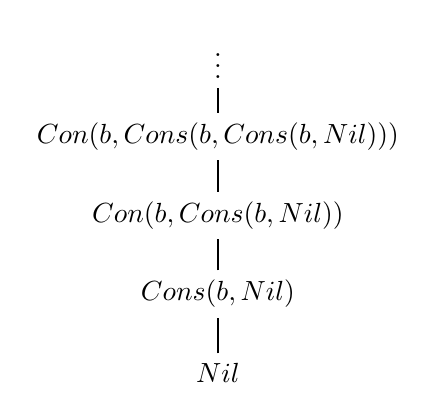
\begin{tikzpicture}                                   
	\node (a) at (0,3) {$\vdots$};                        
	\node (b) at (0,2) {$Con(b, Cons(b, Cons(b, Nil)))$}; 
	\node (c) at (0,1) {$Con(b, Cons(b, Nil))$};          
	\node (d) at (0,0) {$Cons(b, Nil)$};                  
	\node (min) at (0,-1) {$Nil$};                        
	\draw [thick](min) -- (d) -- (c) -- (b) -- (a);       
	\end{tikzpicture}                                     
\end{align*}
In this case, the structural induction of the \ttt{MyListBool} algebra data type grows in a linear-deep way. However, that \textit{easy} grow is not the only one.\\\\
%%
All right, let's take a look now at the \ttt{BSTree} expressions. In this case, we have a recursion definition in the two branches on the second constructor in the definition of \ttt{BSTree} algebra data type. The structural induction derives its shape in two possible nodes, the left one and the right one.\\\\
%%
Let $\Gamma_{BSTree}$ be the set of expressions that define the structure of an element in the \ttt{BSTree} type.
\begin{eqnarray*}
	\Gamma_{BSTree} & = & \{ Nil, \tav T(n, Nil, \; Nil), \\
	&& \tav T(n, \; T(n, Nil, \; Nil), \; Nil), \tav T(n, Nil, \; T(n, Nil, \; Nil)), \tav  \\
	&& \tav T(n, T(n, \; Nil, \; Nil), \; T(n, Nil, \; Nil)), \; \ldots \; \} \tav \tav n \in \ttt{Int}
\end{eqnarray*}
%%
Therefore, $(\Gamma_{BSTree}, \preceq)$ is a poset, where $Nil$ is the minimal element.
\begin{align*}
	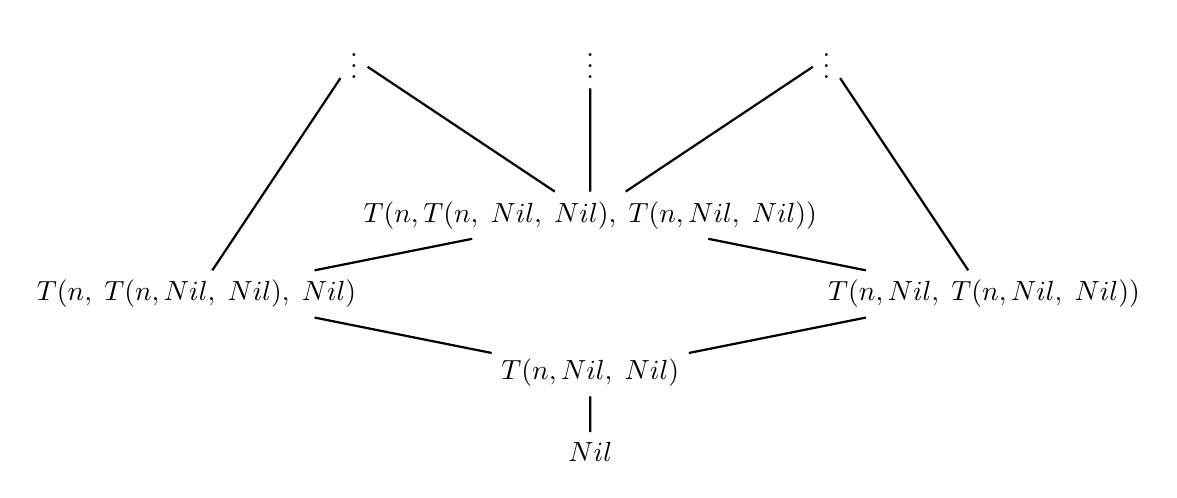
\begin{tikzpicture}                                                       
	\node (a3) at (3,4) {$\vdots$};                                           
	\node (a2) at (0,4) {$\vdots$};                                           
	\node (a1) at (-3,4) {$\vdots$};                                          
	\node (c2) at (0,2) {$T(n, T(n, \; Nil, \; Nil), \; T(n, Nil, \; Nil))$}; 
	\node (c3) at (5,1) {$T(n, Nil, \; T(n, Nil, \; Nil))$};                  
	\node (c1) at (-5,1) {$T(n, \; T(n, Nil, \; Nil), \; Nil)$};              
	\node (d) at (0,0) {$T(n, Nil, \; Nil)$};                                 
	\node (min) at (0,-1) {$Nil$};                                            
	\draw [thick](min) -- (d) -- (c1) -- (c2) -- (a2);                        
	\draw [thick](c1) -- (a1);                                                
	\draw [thick](c3) -- (a3);                                                
	\draw [thick](c2) -- (a3);                                                
	\draw [thick](d) -- (c3) -- (c2) -- (a1);                                 
	\end{tikzpicture}                                                         
\end{align*}
So, the concept of boundaries is not clear and, the more complex the structure more difficult defining the boundaries. In the two examples shown before, is confusing to get the idea of \textit{HOW} grow but it seems that is easy to identify who is the minimal structure right? Both cases are the $Nil$ element. However, what happens with the \ttt{SomeWeird} algebra data type introduced in the last section?\\\\
%%
Here, we have a recursion definition in the two branches on the fourth constructor in the definition of \ttt{SomeWeird} algebra data type. Similar to the \ttt{BSTree} algebra data type, the structural induction derives its shape in two possible nodes, the left one and the right one. However, in this case, we have two '$Nil$' elements: $Nil1$ and $Nil2$. Moreover, we have a third \textit{intermediate} structure $Some$.\\\\
%%
Let $\Gamma_{SomeWeird}$ be the set of expressions that define the structure of an element in the \ttt{SomeWeird} type.
\begin{eqnarray*}
	\Gamma_{SomeWeird} & = & \{ Nil1, \tav Nil2, \tav Some(n), \\
	&& \tav Weird(Nil1, \; Nil1, \; b), \tav Weird(Nil1, \; Nil2, \; b), \\
	&& \tav Weird(Nil2, \; Nil1, \; b), \tav Weird(Nil2, \; Nil2, \; b),  \\
	&& \tav Weird(Nil1, \; Some(n), \; b), \tav Weird(Nil2, \; Some(n), \; b), \; \ldots \; \} \tav \tav n \in \ttt{Int} \tav b \in \ttt{Bool}
\end{eqnarray*}
%%
Therefore, $(\Gamma_{SomeWeird}, \preceq)$ is a poset, where $Nil1$ and $Nil2$ are the minimal elements. Therefore, it wasn't also clear who the minimal element was (in fact, we see there may be several).\\\\
%%
In order to define a general definition of boundary or a well-known structure \textit{size} concept for getting a good-enough space of solutions that hold and providing us completeness in a systematic way, we need to identify those scenarios where an algebra data type is defined recursively and keep in mind the concept of induction. More precisely, mathematical induction over natural numbers or \textit{recursion}, and structural induction. We will see how recursion will help us to control our concept of \textit{size}, and the structural induction will help us to identify which ones are the minimal elements in the poset of the algebra data type expressions.\\
%%

Of course, this is not the only solution. There are a lot of ways to implement the concept of \textit{size} in Prolog, we will show an approach that fits so well with our work and more important: it will be built following the syntax of Haskell's formal grammar, getting consistency between our implementation and the mechanism that we have been defining.\\\\
\pagebreak

Let $\mathcal{H}$, $\mathcal{P}$ be the set of well-defined expressions in Haskell and Prolog, respectively. Let $\psi$ be our syntax-translate mechanism function defined before. We can define $\phi$ a refinement of the function $\psi$ that sends $\mathcal{H}_{\ttt{ADT}} \subsetneq \mathcal{H}$, the subset of well-defined algebra data types expressions in Haskell, to Prolog expressions as follow: $$\phi: \mathcal{H}_{\ttt{ADT}} \longrightarrow \mathcal{P} $$
%%
\begin{align*}
	\ttt{data} \tav tycon \tav \tau_1 \tav \tau_2 \tav \ldots \tav \tau_k 	= & \tav con_1 \tav \alpha_{1,1} \tav \alpha_{1,2} \tav \ldots \tav \alpha_{1,k_1} \tav | &   &   \\
	                                                                         & \tav con_2 \tav \alpha_{2,1} \tav \alpha_{2,2} \tav \ldots \tav \alpha_{2,k_2} \tav | &   &   \\
	                                                                         & \tav \ldots \tav                                                                      &   &   \\
	                                                                         & \tav con_n \tav \alpha_{n,1} \tav \alpha_{n,2} \tav \ldots \tav \alpha_{n,k_n} \tav | &   &   \\
\end{align*}
$$\SLongdownarrow \phi$$
\begin{align*}
	\ttt{rule}_{1}^{0}: \tav \_ tycon (N_{1}^{0}, \tav \_ con_1(X_{1,1}, \tav \ldots, \tav X_{1,k_1})) :-
	  & \tav base(Z_{1,1}),                                             &   &   \\
	  & \tav \ldots                                                     &   &   \\
	  & \tav base(Z_{1,k_1}),                                           &   &   \\
	  & \tav pred_{1, 1}(Z_{1,1}, \tav X_{1,1}),                        &   &   \\
	  & \tav pred_{1, 2}(Z_{1,2}, \tav X_{1,2}),                        &   &   \\
	  & \tav \ldots \tav                                                &   &   \\
	  & \tav pred_{1, k_1}(Z_{1,k_1}, \tav X_{1,k_1}).                  &   &   \\
	\\
	\ttt{rule}_1: \tav \_ tycon (N_1, \tav \_ con_1(X_{1,1}, \tav \ldots, \tav X_{1,k_1})) :-
	  & \tav N_1 > N_{1}^{0},                                           &   &   \\
	  & \tav Nr_1 \tav \ttt{is} \tav N_1 - 1,                           &   &   \\
	  & \tav states_1(Nr_1, \tav W_{1,1}, \tav \ldots, \tav W_{1,k_1}), &   &   \\
	  & \tav pred_{1, 1}(W_{1,1}, \tav X_{1,1}),                        &   &   \\
	  & \tav pred_{1, 2}(W_{1,2}, \tav X_{1,2}),                        &   &   \\
	  & \tav \ldots \tav                                                &   &   \\
	  & \tav pred_{1, k_1}(W_{1,k_1}, \tav X_{1,k_1}).                  &   &   \\
	\ttt{rule}_{2}^{0}: \tav \_ tycon (N_{2}^{0}, \tav \_ con_2(X_{2,1}, \tav \ldots, \tav X_{2,k_2})) :-
	  & \tav base(Z_{2,1}),                                             &   &   \\
	  & \tav \ldots                                                     &   &   \\
	  & \tav base(Z_{2,k_2}),                                           &   &   \\
	  & \tav pred_{2, 1}(Z_{2,1}, \tav X_{2,1}),                        &   &   \\
	  & \tav pred_{2, 2}(Z_{2,2}, \tav X_{2,2}),                        &   &   \\
	  & \tav \ldots \tav                                                &   &   \\
	  & \tav pred_{2, k_2}(Z_{2,k_2}, \tav X_{2,k_2}).                  &   &   \\
	\\
	\ttt{rule}_2: \tav \_ tycon (N_2, \tav \_ con_1(X_{2,1}, \tav \ldots, \tav X_{2,k_2})) :-
	  & \tav N_2 > N_{2}^{0},                                           &   &   \\
	  & \tav Nr_2 \tav \ttt{is} \tav N_2 - 1,                           &   &   \\
	  & \tav states_2(Nr_2, \tav W_{2,1}, \tav \ldots, \tav W_{2,k_2}), &   &   \\
	  & \tav pred_{2, 1}(W_{2,1}, \tav X_{2,1}),                        &   &   \\
	  & \tav pred_{2, 2}(W_{2,2}, \tav X_{2,2}),                        &   &   \\
	  & \tav \ldots \tav                                                &   &   \\
	  & \tav pred_{2, k_2}(W_{2,k_2}, \tav X_{2,k_2}).                  &   &   
\end{align*}
$$\vdots$$
\begin{align*}
	\ttt{rule}_{n}^{0}: \tav \_ tycon (N_{n}^{0}, \tav \_ con_n(X_{n,1}, \tav \ldots, \tav X_{n,k_n})) :-
	  & \tav base(Z_{n,1}),                                             &   &   \\
	  & \tav \ldots                                                     &   &   \\
	  & \tav base(Z_{n,k_n}),                                           &   &   \\
	  & \tav pred_{n, 1}(Z_{n,1}, \tav X_{n,1}),                        &   &   \\
	  & \tav pred_{n, 2}(Z_{n,2}, \tav X_{n,2}),                        &   &   \\
	  & \tav \ldots \tav                                                &   &   \\
	  & \tav pred_{n, k_n}(Z_{n,k_n}, \tav X_{n,k_n}).                  &   &   \\
	\\
	\ttt{rule}_n: \tav \_ tycon (N_n, \tav \_ con_n(X_{n,1}, \tav \ldots, \tav X_{n,k_n})) :-
	  & \tav N_n > N_{n}^{0},                                           &   &   \\
	  & \tav Nr_n \tav \ttt{is} \tav N_n - 1,                           &   &   \\
	  & \tav states_n(Nr_n, \tav W_{n,1}, \tav \ldots, \tav W_{n,k_n}), &   &   \\
	  & \tav pred_{n, 1}(W_{n,1}, \tav X_{n,1}),                        &   &   \\
	  & \tav pred_{n, 2}(W_{n,2}, \tav X_{n,2}),                        &   &   \\
	  & \tav \ldots \tav                                                &   &   \\
	  & \tav pred_{n, k_n}(W_{n,k_n}, \tav X_{n,k_n}).                  &   &   \\
\end{align*}
%%
where:
%%
\begin{itemize}
	\item Let $tycon$ be the algebra data type. We define $\Gamma_{tycon}$ as the set of expressions that define the structure of the elements belonging to $tycon$ type and let's consider the binary operation $\preceq$ defined as, for all $e_1$, $e_2$ two expressions, we say that $e_1 \preceq e_2$ if the expression of $e_1$ is a subexpression contained in the expression $e_2$. Then, we can say that $(\Gamma_{tycon}, \preceq)$ is a poset.
	      %%
	\item For all $con_i$ with $i \in \{1, \ldots, n \}$, there exist two $\ttt{rule}_{i}^{0}$ and $\ttt{rule}_i$ Prolog rules that hold and generate the corresponding translated expression from the Haskell's ADT constructor $i$. The rule $\ttt{rule}_{i}^{0}$ represents the base case in the structural induction for the constructor $con_i$ and $\ttt{rule}_i$ represents the structural induction scenario.\\\\
	      %%
	      In the case of the ADT constructor, $con_i$ doesn't have any component $\alpha_{i,j}$ or for all $j \in \{1, \ldots, k_i \}$ there is no exists any $\alpha_{i,j}$ with recursive type, therefore we can omit the inductive $\ttt{rule}_i$.
	\item For all $con_i$ with $i \in \{1, \ldots, n \}$, there exists a $N_{i}^{0} \in \mathbb{N}$, that represents the minimal \textit{size} (on our \textit{size} concept) of the constructor $con_i$. It will be the base case in the \textit{recursion}.\\\\
	      %%
	      In case of the ADT constructor $con_i$ doesn't have any component $\alpha_{i,j}$ or for all $j \in \{1, \ldots, k_i \}$ there is no exists any $\alpha_{i,j}$ with recursive type, therefore we can define $N_{i}^{0} = 0$.
	      %%
	\item For all $con_i$ with $i \in \{1, \ldots, n \}$, there exists a variable $N_i$ in Prolog, that represents the symbolic variable which will be used to do the recursion scenario from the base case $N_{i}^{0} \in \mathbb{N}$, that is, $N_i$ represent the $m \in \mathbb{N}$ such that if $m > N_{i}^{0}$ implies $rule_i$ hold.
	\item There exists a fact $base$ such that for all $i \in \{1, \ldots, n \}$, $base(N_{i}^{0})$ holds.
	\item For all $\alpha_{i,j}$ with $(i,j) \in \{1, \ldots, n \} \times \{1, \ldots, k_i \}$, there exists a variable $Z_{i,j}$ in Prolog, that represents the symbolic variable for the generation of the base case number in the recursion steps, $N_{i}^{0}$, for the position $j$ in the constructor $i$ which is the Haskell type $\alpha_{i,j}$ in the Haskell's ADT definition.\\\\
	      %%
	      Hence, getting the natural number which represents the minimal \textit{size} (on our \textit{size} concept) of the constructor $j$, we will obtain the expression of the minimal element that the constructor $con_i$ can build.
	\item Let $m \in \mathbb{N}$ be, with $m > N_{i}^{0}$. For all $\alpha_{i,j}$ with $(i,j) \in \{1, \ldots, n \} \times \{1, \ldots, k_i \}$, there exists a variable $W_{i,j}$ in Prolog, that represents the symbolic variable for the generation of the natural $s \in [N_{i}^{0}, m )$ which represent the \textit{size} equal $s$ (on our \textit{size} concept); and a predicate $state_{i}$ such that $states_i(s, \; W_{i,1}, \; \ldots, \; W_{i,k_i})$ holds $\Longleftrightarrow $ for all $b,b' \in \{1, \ldots, k_i \}$,  $W_{i,b}=W_{i,b'} \Rightarrow b = b'$.\\\\
		      %%
		      For this approach, we can implement the functions $state_i$ as:
		      \begin{align*}
		      	state_i(Nr_i, \tav W_{i,1}, \tav \ldots, \tav W_{i, k_i}) :-
		      	  & \tav cases(Nr_i, W_{i,1}),                          &   &   \\
		      	  & \tav cases(Nr_i, W_{i,2}),                          &   &   \\
		      	  & \tav \vdots                                         &   &   \\
		      	  & \tav cases(Nr_i, W_{i,k_i}),                        &   &   \\
		      	  & \tav diff_i(W_{i,1}, \tav \ldots, \tav W_{i, k_i}). &   &   \\\\
		      \end{align*}
		      where
		      \begin{align*}
		      	  & cases(\_, Y) :- \tav base(Y). &   & diff_i(X, \tav \kldots{$k_i$}\;, \tav X) :- \tav base(X), \; !, \; \ttt{fail}. \\
		      	  & cases(X, X).                  &   & diff_i(W_{i,1}, \tav \ldots, \tav W_{i, k_i}).                                 
		      \end{align*}
		      With that, we can obtain an intermediate expression with \textit{size} $s$ in the poset $(\Gamma_{tycon}, \preceq)$. An expression strictly belongs with respect $\preceq$ relation, between the $rule_{i}^{0}$ generate (i.e. the base case in the structural induction) and that one $rule_i$ generate, in the position $j$ from the constructor $i$. Shortly, the expression of the element with \textit{size} $s$ that the constructor $con_i$ can build.
		      %%
	\end{itemize}
	%%
	\subsection{Examples} \label{ch:monomorphic-bounded-types-examples}
	%%
	%%
	\begin{example}[MyListBool]
		Let's suppose the following Haskell ADT definition:
		\lstinputlisting[language=Haskell, label=mylistbool-haskell-monotype]{code/chapter3/monotypes/haskell/mylistbool-monotype.hs}
		Using $\psi$, in the las examples \ref{ch:monomorphic-types-examples} we obtain:
		%%
		\lstinputlisting[language=Prolog, label=mylistbool-prolog-monotype]{code/chapter3/monotypes/prolog/mylistbool-monotype.pl}
		%%
		Now, if we use the newer refinement function $\phi$:
		\begin{itemize}
			\item Let $\Gamma_{MyListBool}$ the set of expressions that define the structure of an element in the \ttt{MyListBool} type. $$\Gamma_{MyListBool} = \{ Nil, \tav Cons(b, Nil), \tav Cons(b, Cons(b, Nil)), \; \ldots \} \tav \tav b \in \ttt{Bool}$$
			      %%
			      We can consider $(\Gamma_{MyListBool}, \preceq)$ that is a poset.
			\item As we have two consutrctor $con_1$ and $con_2$, therefore we have four rules instead, $\ttt{rule}_{1}^{0}$, $\ttt{rule}_1$, $\ttt{rule}_{2}^{0}$ and $\ttt{rule}_2$.
			\item As \ttt{Nil} doesn't have any type in its definition, that is, there is not any $\alpha_{1,j}$ in its Haskell definition. In fact, by using $\phi$ we know that $\ttt{rule}_1$ is a fact \ttt{mylistbool(nil)}, therefore we don't need the $\ttt{rule}_1$ (because we won't do recursion on \ttt{nil}) and we can consider $N_{1}^{0} = 0$, which means, we will consider $Nil$ as the minimal structure in \ttt{MyListBool} with respect our \textit{size} concept.\\\\
			      %%
			      For the second constructor, there exists two $\alpha_{2,1}$ and $\alpha_{2,2}$ related to the expression \ttt{Cons Bool MyListBool}, that is $\alpha_{2,1} = \ttt{Bool}$ and $\alpha_{2,2} = \ttt{MyListBool}$, so here we have to do structural induction in one place: $\alpha_{2,2}$.\\\\
			      %%
			      Therefore, there exists a natural $N_{2}^{0}$, in this case $N_{2}^{0} = 1$, and a variables $Z_{2,2}$ such that $\ttt{rule}_{2}^{0}$ holds and is defined as follow:
			      \begin{flalign*}
			      	\ttt{rule}_{2}^{0}: \tav mylistbool (N_{2}^{0}, \tav t(X_{2,1}, \tav X_{2,2})) :-
			      	& \tav base(Z_{2,2}), && \\
			      	& \tav gen_{\ttt{Bool}}(X_{2,1}), && \\
			      	& \tav mylistbool(Z_{2,2}, \tav X_{2,2}), &&
			      \end{flalign*}
			      This means that $\ttt{rule}_{2}^{0}$ will generate our structural induction base case over the constructor \ttt{cons} and we will obtains those elements with size $N_{2}^{0} = 1$. Also, there exists $N_{2}$ and $W_{2,2}$ variables such that $\ttt{rule}_{2}$ holds and is defined as follow:
			      \begin{flalign*}
			      	\ttt{rule}_{2}: \tav mylistbool (N_{2}, \tav t(X_{2,1}, \tav X_{2,2})) :-
			      	& \tav N_{2} > N_{2}^{0}, && \\
			      	& \tav Nr_{2} \tav \ttt{is} \tav N_{2} - 1, && \\
			      	& \tav states_2(Nr_{2}, \tav W_{2,2}), && \\
			      	& \tav gen_{\ttt{Bool}}(X_{2,1}), && \\
			      	& \tav mylistbool(W_{2,2}, \tav X_{2,2}), &&
			      \end{flalign*}
		\end{itemize}
		So finally, we can translate the Haskell definition shown above to the following Prolog program:\\
		\lstinputlisting[language=Prolog, label=mylistbool-prolog-monotype-boundary]{code/chapter3/monotypes-boundary/mylistbool-boundary.pl}
		Now, if you type \ttt{mylistbool(N, X)} in the Prolog's CLI, you will get a set of valid \ttt{MyListBool} generated value which holds the completeness we have been searching for.\\\\
		%%
		For instance:
		\begin{itemize}
			\item Let $\ttt{N} = 0$, our program returns:
			      \begin{flalign*}
			      	&\ttt{nil} &
			      \end{flalign*}
			\item Let $\ttt{N} = 1$, our program returns:
			      \begin{flalign*}
			      	&\ttt{cons(true, nil)} & \\
			      	&\ttt{cons(false, nil)} &
			      \end{flalign*}
			\item Let $\ttt{N} = 2$, our program returns:
			      \begin{flalign*}
			      	&\ttt{cons(true, cons(true, nil))}&\\
			      	&\ttt{cons(true, cons(false, nil))}&\\
			      	&\ttt{cons(false, cons(true, nil))}&\\
			      	&\ttt{cons(false, cons(false, nil))}&\\
			      \end{flalign*}
		\end{itemize}
	\end{example}
	%%
	\begin{example}[Binary Search Tree]
		Let's suppose the following Haskell ADT definition:
		\lstinputlisting[language=Haskell, label=bst-haskell-monotype]{code/chapter3/monotypes/haskell/bst-monotype.hs}
		Using $\psi$, in the las examples \ref{ch:monomorphic-types-examples} we obtain:
		%%
		\lstinputlisting[language=Prolog, label=bst-prolog-monotype]{code/chapter3/monotypes/prolog/bst-monotype.pl}
		%%
		Now, if we use the newer refinement function $\phi$:
		\begin{itemize}
			\item Let $\Gamma_{BSTree}$ the set of expressions that define the structure of an element in the \ttt{BSTree} type.
			      \begin{eqnarray*}
			      	\Gamma_{BSTree} & = & \{ Nil, \tav T(n, Nil, \; Nil), \\
			      	&& \tav T(n, \; T(n, Nil, \; Nil), \; Nil), \tav T(n, Nil, \; T(n, Nil, \; Nil)), \tav  \\
			      	&& \tav T(n, T(n, \; Nil, \; Nil), \; T(n, Nil, \; Nil)), \; \ldots \; \} \tav \tav n \in \ttt{Int}
			      \end{eqnarray*}
			      %%
			      We can consider $(\Gamma_{BSTree}, \preceq)$ that is a poset.
			\item As we have two consutrctor $con_1$ and $con_2$, therefore we have four rules instead, $\ttt{rule}_{1}^{0}$, $\ttt{rule}_1$, $\ttt{rule}_{2}^{0}$ and $\ttt{rule}_2$.
			\item As \ttt{Nil} doesn't have any type in its definition, that is, there is not any $\alpha_{1,j}$ in its Haskell definition. In fact, by using $\phi$ we know that $\ttt{rule}_1$ is a fact \ttt{bstree(nil)}, therefore we don't need the $\ttt{rule}_1$ (because we won't do recursion on \ttt{nil}) and we can consider $N_{1}^{0} = 0$, which means, we will consider $Nil$ as the minimal structure in \ttt{BSTree} with respect our \textit{size} concept.\\\\
			      %%
			      For the second constructor, there exists three $\alpha_{2,1}$, $\alpha_{2,2}$ and $\alpha_{2,3}$ related to the expression \ttt{T Int BSTree BSTree}, that is $\alpha_{2,1} = \ttt{Int}$, $\alpha_{2,2} = \ttt{BSTree}$ and $\alpha_{2,3} = \ttt{BSTree}$, so here we have to do structural induction in two places: $\alpha_{2,2}$ and $\alpha_{2,3}$.\\\\
			      %%
			      Therefore, there exists a natural $N_{2}^{0}$, in this case $N_{2}^{0} = 1$; two variables $Z_{2,2}$ and $Z_{2,3}$ such that $\ttt{rule}_{2}^{0}$ holds and is defined as follow:
			      \begin{flalign*}
			      	\ttt{rule}_{2}^{0}: \tav bstree (N_{2}^{0}, \tav t(X_{2,1}, \tav X_{2,2}, \tav, X_{2,3})) :-
			      	& \tav base(Z_{2,2}), && \\
			      	& \tav base(Z_{2,3}), && \\
			      	& \tav gen_{\ttt{Int}}(X_{2,1}), && \\
			      	& \tav bstree(Z_{2,2}, \tav X_{2,2}), && \\
			      	& \tav bstree(Z_{2,3}, \tav X_{2,3}). && \\
			      \end{flalign*}
			      This means that $\ttt{rule}_{2}^{0}$ will generate our structural induction base case over the constructor \ttt{t} and we will obtains those elements with size $N_{2}^{0} = 1$. Also, there exists $N_{2}$, $W_{2,2}$ and $W_{2,3}$ variables such that $\ttt{rule}_{2}$ holds and is defined as follow:
			      \begin{flalign*}
			      	\ttt{rule}_{2}: \tav bstree (N_{2}, \tav t(X_{2,1}, \tav X_{2,2}, \tav, X_{2,3})) :-
			      	& \tav N_{2} > N_{2}^{0}, && \\
			      	& \tav Nr_{2} \tav \ttt{is} \tav N_{2} - 1, && \\
			      	& \tav states_2(Nr_{2}, \tav W_{2,2}, \tav W_{2,3}), && \\
			      	& \tav gen_{\ttt{Int}}(X_{2,1}), && \\
			      	& \tav bstree(W_{2,2}, \tav X_{2,2}), && \\
			      	& \tav bstree(W_{2,3}, \tav X_{2,3}). && \\
			      \end{flalign*}
		\end{itemize}
		So finally, we can translate the Haskell definition shown above to the following Prolog program:\\
		\lstinputlisting[language=Prolog, label=binary-search-tree-prolog-monotype-boundary]{code/chapter3/monotypes-boundary/bst-boundary.pl}
		Now, if you type \ttt{bstree(N, X)} in the Prolog's CLI, you will get a set of valid \ttt{BSTree} generated values which hold the completeness we have been searching for.\\\\
		%%
		For instance:
		\begin{itemize}
			\item Let $\ttt{N} = 0$, our program returns:
			      \begin{flalign*}
			      	&\ttt{nil} &
			      \end{flalign*}
			\item Let $\ttt{N} = 1$, our program returns:
			      \begin{flalign*}
			      	&\ttt{t(-245966722, nil, nil)} &
			      \end{flalign*}
			\item Let $\ttt{N} = 2$, our program returns:
			      \begin{flalign*}
			      	&\ttt{t(208235124, nil, t(158289014, nil, nil))}&\\
			      	&\ttt{t(308826753, t(-184602937, nil, nil), nil)}&\\
			      	&\ttt{t(302818108, t(324337197, nil, nil), t(295232001, nil, nil))}& \\
			      \end{flalign*}
		\end{itemize}
	\end{example}
	%%
	\begin{example}[SomeWeird]
		Let's suppose the following Haskell ADT definition:
		\lstinputlisting[language=Haskell, label=someweird-haskell-monotype]{code/chapter3/monotypes/haskell/someweird-monotype.hs}
		Using $\psi$, in the las examples \ref{ch:monomorphic-types-examples} we obtain:
		%%
		\lstinputlisting[language=Prolog, label=someweird-prolog-monotype]{code/chapter3/monotypes/prolog/someweird-monotype.pl}
		%%
		Now, if we use the newer refinement function $\phi$:
		\begin{itemize}
			\item Let $\Gamma_{SomeWeird}$ the set of expressions that define the structure of an element in the \ttt{SomeWeird} type.
			      \begin{eqnarray*}
			      	\Gamma_{SomeWeird} & = & \{ Nil1, \tav Nil2, \tav Some(n), \\
			      	&& \tav Weird(Nil1, \; Nil1, \; b), \tav Weird(Nil1, \; Nil2, \; b), \\
			      	&& \tav Weird(Nil2, \; Nil1, \; b), \tav Weird(Nil2, \; Nil2, \; b),  \\
			      	&& \tav Weird(Nil1, \; Some(n), \; b), \tav Weird(Nil2, \; Some(n), \; b), \; \ldots \; \} \\
			      	&& \tav n \in \ttt{Int} \tav b \in \ttt{Bool}
			      \end{eqnarray*}
			      %%
			      We can consider $(\Gamma_{SomeWeird}, \preceq)$ that is a poset.
			\item As we have four consutrctors $con_1$, $con_2$, $con_3$ and $con_4$, therefore we have eight rules instead, $\ttt{rule}_{1}^{0}$, $\ttt{rule}_1$, $\ttt{rule}_{2}^{0}$, $\ttt{rule}_2$, $\ttt{rule}_{3}^{0}$, $\ttt{rule}_3$, $\ttt{rule}_{4}^{0}$ and $\ttt{rule}_4$.
			\item As both \ttt{Nil1} and \ttt{Nil2} don't have any type in their definitions, that is, there is not any $\alpha_{1,j}$ and $\alpha_{2,j}$ in their Haskell definition, respectively. In fact, by using $\phi$ we know that both $\ttt{rule}_1$ and $\ttt{rule}_2$ are facts \ttt{someweird(nil1)} and \ttt{someweird(nil1)}; therefore we don't need neither $\ttt{rule}_1$ nor $\ttt{rule}_2$ (because we won't do recursion on \ttt{nil1} nor \ttt{nil2}) and we can consider $N_{1}^{0} = 0$ and $N_{2}^{0} = 0$, which means, we will consider both \ttt{Nil1} and \ttt{Nil2} as the minimal structures in \ttt{SomeWeird} with respect our \textit{size} concept.\\\\
			      %%
			      For the third constructor, there exists a $\alpha_{3,1}$  related to the expression \ttt{Some Int}, that is $\alpha_{3,1} = \ttt{Int}$. However, we won't do structural induction on that. Therefore, we work similarly as both \ttt{Nil1} and \ttt{Nil2}. That is, we can consider $N_{3}^{0} = 0$, which means, we will consider \ttt{Some Int} as another minimal structure in \ttt{SomeWeird} concerning our \textit{size} concept. So, at this moment, we have three minimal elements: \ttt{Nil1}, \ttt{Nil2} and \ttt{Some Int}.\\\\
			      %%
			      For the fourth constructor, there exists three $\alpha_{4,1}$, $\alpha_{4,2}$ and $\alpha_{4,3}$ related to the expression \ttt{Weird SomeWeird SomeWeird Bool}, that is $\alpha_{4,1} = \ttt{SomeWeird}$, $\alpha_{4,2} = \ttt{SomeWeird}$ and $\alpha_{4,3} = \ttt{Bool}$, so here we have to do structural induction in two places: $\alpha_{4,1}$ and $\alpha_{4,2}$.\\\\
			      %%
			      Therefore, there exists a natural $N_{4}^{0}$, in this case $N_{4}^{0} = 1$; two variables $Z_{4,1}$ and $Z_{4,2}$ such that $\ttt{rule}_{4}^{0}$ holds and is defined as follow:
			      \begin{flalign*}
			      	\ttt{rule}_{4}^{0}: \tav someweird (N_{4}^{0}, \tav weird(X_{4,1}, \tav X_{4,2}, \tav, X_{4,3})) :-
			      	& \tav base(Z_{4,1}), && \\
			      	& \tav base(Z_{4,2}), && \\
			      	& \tav someweird(Z_{4,1}, \tav X_{4,1}), && \\
			      	& \tav someweird(Z_{4,2}, \tav X_{4,2}), && \\
			      	& \tav gen_{\ttt{Bool}}(X_{4,3}), &&
			      \end{flalign*}
			      This means that $\ttt{rule}_{4}^{0}$ will generate our structural induction base case over the constructor \ttt{weird} and we will obtains those elements with size $N_{4}^{0} = 1$. Also, there exists $N_{4}$, $W_{4,1}$ and $W_{4,2}$ variables such that $\ttt{rule}_{4}$ holds and is defined as follow:
			      \begin{flalign*}
			      	\ttt{rule}_{4}: \tav someweird (N_{4}, \tav weird(X_{4,1}, \tav X_{4,2}, \tav, X_{4,3})) :-
			      	& \tav N_{4} > N_{4}^{0}, && \\
			      	& \tav Nr_{4} \tav \ttt{is} \tav N_{4} - 1, && \\
			      	& \tav states_4(Nr_{4}, \tav W_{4,1}, \tav W_{4,2}), && \\
			      	& \tav someweird(W_{4,1}, \tav X_{4,1}), && \\
			      	& \tav someweird(W_{4,2}, \tav X_{4,2}), && \\
			      	& \tav gen_{\ttt{Bool}}(X_{4,3}), &&
			      \end{flalign*}
		\end{itemize}
		So finally, we can translate the Haskell definition shown above to the following Prolog program:\\
		\lstinputlisting[language=Prolog, label=someweird-prolog-monotype-boundary]{code/chapter3/monotypes-boundary/someweird-boundary.pl}
		Now, if you type \ttt{someweird(N, X)} in the Prolog's CLI, you will get a set of valid \ttt{SomeWeird} generated values which hold the completeness we have been searching for.\\\\
		%%
		For instance:
		\begin{itemize}
			\item Let $\ttt{N} = 0$, our program returns:
			      \begin{flalign*}
			      	&\ttt{nil1}&\\
			      	&\ttt{nil2}&\\
			      	&\ttt{some(371056659)}&\\
			      \end{flalign*}
			\item Let $\ttt{N} = 1$, our program returns:
			      \begin{flalign*}
			      	&\ttt{weird(nil1, nil1, true)}&\\
			      	&\ttt{weird(nil1, nil1, false)}&\\
			      	&\ttt{weird(nil1, nil2, true)}&\\
			      	&\ttt{weird(nil1, nil2, false)}&\\
			      	&\ttt{weird(nil1, some(-427613704), true)}&\\
			      	&\ttt{weird(nil1, some(-427613704), false)}&\\
			      	&\ttt{weird(nil2, nil1, true)}&\\
			      	&\ttt{weird(nil2, nil1, false)}&\\
			      	&\ttt{weird(nil2, nil2, true)}&\\
			      	&\ttt{weird(nil2, nil2, false)}&\\
			      	&\ttt{weird(nil2, some(-266152950), true)}&\\
			      	&\ttt{weird(nil2, some(-266152950), false)}&\\
			      	&\ttt{weird(some(374335935), nil1, true)}&\\
			      	&\ttt{weird(some(374335935), nil1, false)}&\\
			      	&\ttt{weird(some(374335935), nil2, true)}&\\
			      	&\ttt{weird(some(374335935), nil2, false)}&\\
			      	&\ttt{weird(some(374335935), some(-27052657), true)}&\\
			      	&\ttt{weird(some(374335935), some(-27052657), false)}&\\
			      \end{flalign*}
		\end{itemize}
	\end{example}
	\section{Polymorfism Types}
	We are now in the last problem of our journey: the polymorphism types. Usually, algebra data types are defined by using parameter types that represent the polymorphism. We can obtain a greater set of elements belonging to the ADT type. In particular, we can obtain a set of instances of our ADT for every type that you can use in its implementation. So here, we have to deal with a more abstract level. Therefore, the idea here is the following:\\\\
	%%
	Let's suppose our known definition of Binary Search Tree in Haskell:
	\lstinputlisting[language=Haskell, label=bst-haskell-monotype]{code/chapter3/monotypes/haskell/bst-monotype.hs}
	We need to know what should look like it in a polymorphic approach. So, first of all, let's define its polymorphic version:
	\lstinputlisting[language=Haskell, label=bst-haskell-monotype]{code/chapter3/polymorphic/haskell/bst-polymorphic.hs}
	Now, our Haskell expression depends on a type parameter. Let's take a look at our first Binary Search Tree Prolog implementation results of the syntax-translation mechanism $\psi$ defined in \ref{ch:monomorphic-types}.
	%%
	\lstinputlisting[language=Prolog, label=bst-prolog-monotype]{code/chapter3/monotypes/prolog/bst-monotype.pl}
	%%
	We see that by changing $\ttt{gen\_int}$ for some other more general $gen$ function we could obtain a parametrized generator of types. That is, we can define a newer generator as something like that \ttt{gen(T, X)}, where \ttt{T} is the symbolic variable that parametrises the type.
	%%
	\lstinputlisting[language=Prolog, label=bst-prolog-monotype]{code/chapter3/polymorphic/prolog/bst-draft.pl}
	%%
	However, an algebra data type can be defined using as many representation polymorphic types as it needs. So, we have to generalize it also following the Haskell formal grammar.\\\\
	Let $\mathcal{H}$, $\mathcal{P}$ be the set of well-defined expressions in Haskell and Prolog, respectively. Let $\psi$ be our syntax-translate mechanism function defined in the last section. We can define $\Psi$ a refinement of the function $\psi$ that sends $\mathcal{H}_{\ttt{ADT}} \subsetneq \mathcal{H}$, the subset of well-defined algebra data types expressions in Haskell, to Prolog expressions as follow: $$\Psi: \mathcal{H}_{\ttt{ADT}} \longrightarrow \mathcal{P} $$
	%%
	\begin{align*}
		\ttt{data} \tav tycon \tav \tau_1 \tav \tau_2 \tav \ldots \tav \tau_k 	= & \tav con_1 \tav \alpha_{1,1} \tav \alpha_{1,2} \tav \ldots \tav \alpha_{1,k_1} \tav | &   &   \\
		                                                                         & \tav con_2 \tav \alpha_{2,1} \tav \alpha_{2,2} \tav \ldots \tav \alpha_{2,k_2} \tav | &   &   \\
		                                                                         & \tav \ldots \tav                                                                      &   &   \\
		                                                                         & \tav con_n \tav \alpha_{n,1} \tav \alpha_{n,2} \tav \ldots \tav \alpha_{n,k_n} \tav | &   &   \\
	\end{align*}
	$$\SLongdownarrow \Psi$$
	\begin{align*}
		\ttt{rule}_1: \tav \_ tycon (T_1, \tav T_2, \tav \ldots, \tav T_k, \; \_ con_1(X_{1,1}, \tav \ldots, \tav X_{1,k_1})) :-&
		\tav pred_{1, 1}(\Omega_{1,1}, \tav X_{1,1}), && \\
		  & \tav pred_{1, 2}(\Omega_{1,2}, \tav X_{1,2}),       &   &   \\
		  & \tav \ldots \tav                                    &   &   \\
		  & \tav pred_{1, k_1}(\Omega_{1,k_1}, \tav X_{1,k_1}). &   &   \\
		\\
		\ttt{rule}_2: \tav \_ tycon (T_1, \tav T_2, \tav \ldots, \tav T_k, \; \_ con_2(X_{2,1}, \tav \ldots, \tav X_{2,k_2})) :-&
		\tav pred_{2, 1}(\Omega_{2,1}, \tav X_{2,1}), && \\
		  & \tav pred_{2, 2}(\Omega_{2,2}, \tav X_{2,2}),       &   &   \\
		  & \tav \ldots \tav                                    &   &   \\
		  & \tav pred_{2, k_2}(\Omega_{2,k_2}, \tav X_{2,k_2}). &   &   
	\end{align*}
	$$\vdots$$
	\begin{align*}
		\ttt{rule}_n: \tav \_ tycon (T_1, \tav T_2, \tav \ldots, \tav T_k, \; \_ con_n(X_{n,1}, \tav \ldots, \tav X_{n,k_n})) :-&
		\tav pred_{n, 1}(\Omega_{n,1}, \tav X_{n,1}), && \\
		  & \tav pred_{n, 2}(\Omega_{n,2}, \tav X_{n,2}),       &   &   \\
		  & \tav \ldots \tav                                    &   &   \\
		  & \tav pred_{n, k_n}(\Omega_{n,k_n}, \tav X_{n,k_n}). &   &   \\
	\end{align*}\\
	%%
	where:
	%%
	\begin{itemize}
		\item For all $\tau_i$ with $i \in \{1, \ldots k \}$, there exists a variable $T_i$ in Prolog, that represents the symbolic variable for the type that it will generate.
		      \begin{example}
		      	Let's suppose the polymorphic version of the definition of Either:
		      	\lstinputlisting[language=Haskell, label=either-haskell-monotype]{code/chapter3/polymorphic/haskell/either-polymorphic.hs}
		      	Here, you can see that $\tau_1 = \ttt{a}$, $\tau_2 = \ttt{b}$, therefore there exists two variables, $T_1$ and $T_2$, respectively.\\\\
		      	%%
		      	In our Prolog program, we will define a relationship between some atoms which will represent the type expression in Prolog, concerning its corresponding generation function.\\\\
		      	%%
		      	For example, if we have the \ttt{Either} definition showed above and we want to generate instances for \ttt{Either Unit Bool}, that is $\tau_1 = \ttt{Unit}$, $\tau_2 = \ttt{Bool}$, we will use $T_1 = \ttt{unit}$ and $T_2 = \ttt{bool}$ for getting the correct generation. Of course, it is the standard representation that we have chosen, we could have defined $\ttt{unit\_type}$ and $\ttt{bool\_type}$ instead for representing \ttt{Unit} and \ttt{Bool} in Prolog, respectively.
		      \end{example}
		\item Let $P(\{ T_1 , T_2, \ldots, \; T_k \})$ be the \textit{powerset} of the set of all Prolog types variables. For all $\alpha_{i,j}$ with $(i,j) \in \{1, \ldots n \} \times \{1, \ldots k_i \}$, we define $\Omega_{i,j}$ an element of $P(\{ T_1, T_2, \ldots, \; T_k \})$ as the set of the those Prolog types variables that participate in the definition of $\alpha_{i,j}$ at our Haskell's algebra data type definition.
		      %%
		      \begin{example}
		      	Let's suppose the polymorphic version of the \ttt{SomeWeird} definition:
		      	\lstinputlisting[language=Haskell, label=someweird-haskell-polymorphic]{code/chapter3/polymorphic/haskell/someweird-polymorphic.hs}
		      	Here, $\tau_1 = \ttt{a}$ and $\tau_2=\ttt{b}$, we can define $T_1 = \ttt{A}$ and $T_2=\ttt{B}$
		      	\begin{itemize}
		      		\item As \ttt{Nil1} constructor doesn't require any type to be defined, therefore $\Omega_{1,1} = \emptyset \in P(\{ \ttt{A}, \ttt{B} \})$.
		      		\item As \ttt{Nil2} constructor doesn't require any type to be defined, therefore $\Omega_{2,1} = \emptyset \in P(\{ \ttt{A}, \ttt{B} \})$.
		      		\item As \ttt{Some} constructor requires \ttt{a}, that is, $\alpha_{3,1} = \ttt{a}$ and it needs $\ttt{a}$ to be defined, therefore $\Omega_{3,1} = \{\ttt{A}\} \in P(\{ \ttt{A} , \ttt{B} \})$.
		      		\item As $\ttt{Weird}$ constructor requires both types \ttt{SomeWeird a b} and \ttt{b}, that is, $\alpha_{4,1} = \alpha_{4,2} = \ttt{SomeWeird a b}$ and $\alpha_{4,3} = \ttt{b}$, therefore $\Omega_{4,1} = \Omega_{4,2} = \{\ttt{A}, \ttt{B}\} \in P(\{ \ttt{A} , \ttt{B} \})$ and $\Omega_{4,3} = \{\ttt{B}\} \in P(\{ \ttt{A} , \ttt{B} \})$.
		      	\end{itemize}
		      \end{example}
		\item For all $\alpha_{i,j}$ with $(i,j) \in \{1, \ldots n \} \times \{1, \ldots k_i \}$, there exists a predicate $pred_{i,j}$ that resolve $X_{i,j}$ using $\Omega_{i,j}$.\\\\
		      %%
		      When $\alpha_{i,j}$ is an Haskell's primitive type, that means $\Omega_{i,j} = \{T_{\omega_{i,j}}\}$ with $T_{\omega_{i,j}} \in \{ T_1 , T_2, \ldots T_k \}$, the predicate $pred_{i,j}$ can be defined as the $gen$ generation function. That is, $pred_{i,j}(\Omega_{i,j}, X_{i,j}) \equiv gen(T_{\omega_{i,j}}, X_{i,j})$, being the $gen$ generation function our new Prolog rule that generates a value of type $\tau_{\omega_{i,j}} \in \{ \tau_1, \tau_2, \ldots \tau_k \}$.
	\end{itemize}
	\subsection{Generic Polymorphic Types Generator}
	For this work, I provide an implementation of the generic $gen$ generation function of primitive types which generalize by using a type variable as a new parameter. This implementation is not the best efficient one, but it is enough for our purpose. First of all, we define the atoms which will represent the type expression in our Prolog program. That is:
	\begin{equation*}
		\begin{matrix}
			\Psi_{\ttt{Type}}: & \mathcal{H}   & \longrightarrow & \tav \mathcal{P} &   &   &   \\
			                   & \ttt{Char}    & \longrightarrow & \ttt{char}       &   &   &   \\
			                   & \ttt{String}  & \longrightarrow & \ttt{string}     &   &   &   \\
			                   & \ttt{Int}     & \longrightarrow & \ttt{int}        &   &   &   \\
			                   & \ttt{Integer} & \longrightarrow & \ttt{integer}    &   &   &   \\
			                   & \ttt{Double}  & \longrightarrow & \ttt{double}     &   &   &   \\
			                   & \ttt{Bool}    & \longrightarrow & \ttt{bool}       &   &   &   \\
			                   & \ttt{Unit}    & \longrightarrow & \ttt{unit}       &   &   &   \\
		\end{matrix}
	\end{equation*}
	Therefore, we can define the following relationship in Prolog:\\\\
	%%
	Let $gen$ be the function which generates values of primitive types. We can implement in Prolog this function as the following rule:
	\lstinputlisting[language=Prolog, label=gen-types]{code/chapter3/polymorphic/prolog/gen_types.pl}
	So now, we can obtain a boolean value just by typing \ttt{gen(bool, B)}. The last cases $\ttt{rel\_gen}$ are when you want to generate polymorphically by using another non-primitive generator. For instance:\\\\
	%%
	Let's suppose our Prolog program that generates Binary Search Trees from the polymorphic definition.
	%%
	\lstinputlisting[language=Prolog, label=bst-prolog-monotype]{code/chapter3/polymorphic/prolog/bst-draft.pl}
	We want to generate lists of Binary Search Trees. In order to do that, we could just implement the polymorphic version of a generation of lists and use our \ttt{bstree} program:
	\lstinputlisting[language=Prolog, label=polymorphic-lists]{code/chapter3/polymorphic/prolog/list.pl}
	Now, if you type \ttt{list(bstree(unit), 2, X)} in the Prolog's CLI, you will get a valid list of \ttt{BSTree} generated value:
	\begin{align*}
		  & \ttt{[nil, nil]}                                           &   \\
		  & \ttt{[nil, t(unit, nil, nil)]}                             &   \\
		  & \ttt{[nil, t(unit, nil, t(unit, nil, nil))]}               &   \\
		  & \ttt{[nil, t(unit, nil, t(unit, nil, t(unit, nil, nil)))]} &   \\
	\end{align*}
	Of course, you could have used the boundary version of \ttt{bstree} to get more control over the space of solutions.\\\\
	%%
	Finally, we can show many examples using this polymorphic approach. However, before proceeding further, I will provide the refinement of $\phi$ defined in the last section \ref{ch:monomorphic-types-boundaries} with its polymorphic version.
	\subsection{Polymorfism Types with Boundaries}
	%%
	Let $\mathcal{H}$, $\mathcal{P}$ be the set of well-defined expressions in Haskell and Prolog, respectively. Let $\phi$ be our syntax-translate mechanism function defined in the last section. We can define $\Phi$ a refinement of the function $\phi$ that sends $\mathcal{H}_{\ttt{ADT}} \subsetneq \mathcal{H}$, the subset of well-defined algebra data types expressions in Haskell, to Prolog expressions as follow: $$\Phi: \mathcal{H}_{\ttt{ADT}} \longrightarrow \mathcal{P} $$
	%%
	\begin{align*}
		\ttt{data} \tav tycon \tav \tau_1 \tav \tau_2 \tav \ldots \tav \tau_k 	= & \tav con_1 \tav \alpha_{1,1} \tav \alpha_{1,2} \tav \ldots \tav \alpha_{1,k_1} \tav | &   &   \\
		                                                                         & \tav con_2 \tav \alpha_{2,1} \tav \alpha_{2,2} \tav \ldots \tav \alpha_{2,k_2} \tav | &   &   \\
		                                                                         & \tav \ldots \tav                                                                      &   &   \\
		                                                                         & \tav con_n \tav \alpha_{n,1} \tav \alpha_{n,2} \tav \ldots \tav \alpha_{n,k_n} \tav | &   &   \\
	\end{align*}
	$$\SLongdownarrow \Phi$$
	\begin{align*}
		\ttt{rule}_{1}^{0}: \tav \_ tycon (N_{1}^{0}, \tav T_1, \tav T_2, \tav \ldots, \tav T_k, \; \_ con_1(X_{1,1}, \tav \ldots, \tav X_{1,k_1})) :-
		  & \tav base(Z_{1,1}),                                                 &   &   \\
		  & \tav \ldots                                                         &   &   \\
		  & \tav base(Z_{1,k_1}),                                               &   &   \\
		  & \tav pred_{1, 1}(Z_{1,1}, \tav \Omega_{1,1}, \tav X_{1,1}),         &   &   \\
		  & \tav pred_{1, 2}(Z_{1,2}, \tav \Omega_{1,2}, \tav X_{1,2}),         &   &   \\
		  & \tav \ldots \tav                                                    &   &   \\
		  & \tav pred_{1, k_1}(Z_{1,k_1}, \tav \Omega_{1,k_1} \tav X_{1,k_1}).  &   &   \\
		\\
		\ttt{rule}_1: \tav \_ tycon (N_1, \tav T_1, \tav T_2, \tav \ldots, \tav T_k, \; \_ con_1(X_{1,1}, \tav \ldots, \tav X_{1,k_1})) :-
		  & \tav N_1 > N_{1}^{0},                                               &   &   \\
		  & \tav Nr_1 \tav \ttt{is} \tav N_1 - 1,                               &   &   \\
		  & \tav states_1(Nr_1, \tav W_{1,1}, \tav \ldots, \tav W_{1,k_1}),     &   &   \\
		  & \tav pred_{1, 1}(W_{1,1}, \tav \Omega_{1, 1} \tav X_{1,1}),         &   &   \\
		  & \tav pred_{1, 2}(W_{1,2}, \tav \Omega_{1, 2} \tav X_{1,2}),         &   &   \\
		  & \tav \ldots \tav                                                    &   &   \\
		  & \tav pred_{1, k_1}(W_{1,k_1}, \tav \Omega_{1, k_1} \tav X_{1,k_1}). &   &   
	\end{align*}
	$$\vdots$$
	\begin{align*}
		\ttt{rule}_{n}^{0}: \tav \_ tycon (N_{n}^{0}, \tav T_1, \tav T_2, \tav \ldots, \tav T_k, \; \_ con_n(X_{n,1}, \tav \ldots, \tav X_{n,k_n})) :-
		  & \tav base(Z_{n,1}),                                                 &   &   \\
		  & \tav \ldots                                                         &   &   \\
		  & \tav base(Z_{n,k_n}),                                               &   &   \\
		  & \tav pred_{n, 1}(Z_{n,1}, \tav \Omega_{n, 1} \tav X_{n,1}),         &   &   \\
		  & \tav pred_{n, 2}(Z_{n,2}, \tav \Omega_{n, 2} \tav X_{n,2}),         &   &   \\
		  & \tav \ldots \tav                                                    &   &   \\
		  & \tav pred_{n, k_n}(Z_{n,k_n}, \tav \Omega_{n, k_n} \tav X_{n,k_n}). &   &   \\
		\\
		\ttt{rule}_n: \tav \_ tycon (N_n, \tav T_1, \tav T_2, \tav \ldots, \tav T_k, \; \_ con_n(X_{n,1}, \tav \ldots, \tav X_{n,k_n})) :-
		  & \tav N_n > N_{n}^{0},                                               &   &   \\
		  & \tav Nr_n \tav \ttt{is} \tav N_n - 1,                               &   &   \\
		  & \tav states_n(Nr_n, \tav W_{n,1}, \tav \ldots, \tav W_{n,k_n}),     &   &   \\
		  & \tav pred_{n, 1}(W_{n,1}, \tav \Omega_{n, 1} \tav X_{n,1}),         &   &   \\
		  & \tav pred_{n, 2}(W_{n,2}, \tav \Omega_{n, 2} \tav X_{n,2}),         &   &   \\
		  & \tav \ldots \tav                                                    &   &   \\
		  & \tav pred_{n, k_n}(W_{n,k_n}, \tav \Omega_{n, k_n} \tav X_{n,k_n}). &   &   \\
	\end{align*}\\
	%%
	\subsection{Examples} \label{ch:polymorphic-types-examples}
	For the following examples, we will use the polymorphic and bounded approach $\Phi$. Of course, we avoid showing again the auxiliary corresponding function that accompanies the respective Prolog program in order to be briefer.
	\begin{example}[MyList]
		Let's consider the polymorphic version of our \ttt{MyListBool} Haskell ADT definition:
		\lstinputlisting[language=Haskell, label=mylist-haskell-polymorphic]{code/chapter3/polymorphic/haskell/mylist-polymorphic.hs}
		Using $\phi$, in the las examples \ref{ch:monomorphic-bounded-types-examples} we obtain:
		%%
		\lstinputlisting[language=Prolog, label=mylistbool-prolog-monotype-boundary]{code/chapter3/monotypes-boundary/mylistbool-boundary-simplify.pl}
		%%
		Now, if we use the newer refinement function $\Phi$:
		\begin{itemize}
			\item We can see that there exists a $\tau_1$. Therefore there exists a variable, $T_1$.
			\item Here, $\tau_1 = \ttt{a}$ so we can define $T_1 = \ttt{A}$ and consider the poset $P(\{\ttt{A}\})$.
			\item As \ttt{Nil} constructor doesn't require any type to be defined, therefore $\Omega_{1,1} = \emptyset \in P(\{ \ttt{A} \})$. \\\\
			      For the second constructor, there exists two $\alpha_{2,1}$ and $\alpha_{2,2}$ related to the expression \ttt{Cons a (MyList a)}, that is $\alpha_{2,1} = \ttt{a}$ and $\alpha_{2,2} = \ttt{MyList a}$, which both is defined polymorphically, therefore $\Omega_{2,1} = \{\ttt{A}\} \in P(\{ \ttt{A} \})$ and $\Omega_{2,2} = \{\ttt{A}\} \in P(\{ \ttt{A} \})$.
		\end{itemize}
		So finally, we can translate the Haskell definition shown above to the following Prolog program:\\
		\lstinputlisting[language=Prolog, label=mylist-prolog-polymorphic]{code/chapter3/polymorphic/prolog/mylist-polymorphic.pl}
		Now, if you type \ttt{mylist(N, bool, X)} in the Prolog's CLI, you will get a set of valid \ttt{MyList a} with $\ttt{a} := \ttt{Bool}$ generated values which is the same set than the generated one by using our old \ttt{MyListBool} program and holds the completeness we have been searching for.\\
	\end{example}
	%%
	\begin{example}[Binary Search Tree]
		Let's consider the polymorphic version of our \ttt{BSTree} Haskell ADT definition:
		\lstinputlisting[language=Haskell, label=binary-search-tree-haskell-polymorphic]{code/chapter3/polymorphic/haskell/bst-polymorphic.hs}
		Using $\phi$, in the las examples \ref{ch:monomorphic-bounded-types-examples} we obtain:
		%%
		\lstinputlisting[language=Prolog, label=binary-search-tree-prolog-monotype-boundary]{code/chapter3/monotypes-boundary/bst-boundary-simplify.pl}
		%%
		Now, if we use the newer refinement function $\Phi$:
		\begin{itemize}
			\item We can see that there exists a $\tau_1$. Therefore there exists a variable, $T_1$.
			\item Here, $\tau_1 = \ttt{a}$ so we can define $T_1 = \ttt{A}$ and consider the poset $P(\{\ttt{A}\})$.
			\item As \ttt{Nil} constructor doesn't require any type to be defined, therefore $\Omega_{1,1} = \emptyset \in P(\{ \ttt{A} \})$. \\\\
			      For the second constructor, there exists three $\alpha_{2,1}$, $\alpha_{2,2}$ and $\alpha_{2,3}$ related to the expression \ttt{T a (BSTree a) (BSTree a)}, that is $\alpha_{2,1} = \ttt{a}$ and $\alpha_{2,2} = \alpha_{2,3} = \ttt{BSTree a}$, which both is defined polymorphically, therefore $\Omega_{2,1} = \{\ttt{A}\} \in P(\{ \ttt{A} \})$ and $\Omega_{2,2} = \Omega_{2,3} = \{\ttt{A}\} \in P(\{ \ttt{A} \})$.
		\end{itemize}
		So finally, we can translate the Haskell definition shown above to the following Prolog program:\\
		\lstinputlisting[language=Prolog, label=binary-search-tree-prolog-polymorphic]{code/chapter3/polymorphic/prolog/bst-polymorphic.pl}
		Now, if you type \ttt{bstree(N, int, X)} in the Prolog's CLI, you will get a set of valid \ttt{BSTree a} with $\ttt{a} := \ttt{Int}$ generated values which is the same set than the generated one by using our old monomorphic type version of \ttt{BSTree} program and holds the completeness we have been searching for.\\
	\end{example}
	%%
	\begin{example}[SomeWeird]
		Let's consider the polymorphic version of our \ttt{SomeWeird} Haskell ADT definition:
		\lstinputlisting[language=Haskell, label=someweird-haskell-polymorphic]{code/chapter3/polymorphic/haskell/someweird-polymorphic.hs}
		Using $\phi$, in the las examples \ref{ch:monomorphic-bounded-types-examples} we obtain:
		%%
		\lstinputlisting[language=Prolog, label=someweird-prolog-monotype-boundary]{code/chapter3/monotypes-boundary/someweird-boundary-simplify.pl}
		%%
		Now, if we use the newer refinement function $\Phi$:
		\begin{itemize}
			\item We can see that there exists two $\tau_1$ and $\tau_2$. Therefore there exist two variables, $T_1$ and $T_2$.
			\item Here, $\tau_1 = \ttt{a}$ and $\tau_2 = \ttt{b}$ so we can define $T_1 = \ttt{A}$, $T_2 = \ttt{B}$ and consider the poset $P(\{\ttt{A}, \ttt{B}\})$.
			\item As \ttt{Nil1} constructor doesn't require any type to be defined, therefore $\Omega_{1,1} = \emptyset \in P(\{ \ttt{A} \})$. \\\\
			      As \ttt{Nil2} constructor doesn't require any type to be defined, therefore $\Omega_{2,1} = \emptyset \in P(\{ \ttt{A} \})$. \\\\
			      For the third constructor, there exists an $\alpha_{3,1}$ related to the expression \ttt{Some a}, that is $\alpha_{3,1} = \ttt{a}$, which is defined polymorphically, therefore $\Omega_{3,1} = \{\ttt{A}\} \in P(\{ \ttt{A} \})$. \\\\
			      For the fourth constructor, there exists three $\alpha_{4,1}$, $\alpha_{4,2}$ and $\alpha_{4,3}$ related to the expression \ttt{Weird (SomeWeird a) (SomeWeird a) b}, that is $\alpha_{4,1} = \alpha_{4,2} = \ttt{SomeWeird a b}$ and $\alpha_{4,3} = \ttt{b}$, which both is defined polymorphically, therefore $\Omega_{4,1} = \Omega_{4,2} = \{\ttt{A}, \ttt{B}\} \in P(\{ \ttt{A} , \ttt{B} \})$ and $\Omega_{4,3} = \{\ttt{B}\} \in P(\{ \ttt{A} , \ttt{B} \})$.
			      %%
		\end{itemize}
		So finally, we can translate the Haskell definition shown above to the following Prolog program:\\
		\lstinputlisting[language=Prolog, label=someweird-polymorphic]{code/chapter3/polymorphic/prolog/someweird-polymorphic.pl}
		Now, if you type \ttt{someweird(N, int, bool, X)} in the Prolog's CLI, you will get a set of valid \ttt{SomeWeird a b} with $\ttt{a} := \ttt{Int}$ and $\ttt{b} := \ttt{Bool}$ generated values which is the same set than the generated one by using our old monomorphic type version of \ttt{SomeWeird} program and holds the completeness we have been searching for.\\
	\end{example}
	%%
	\subsection{Red-Black Tree}
	Finally, we have the tools to get the Prolog program approach from a Red-Black Tree Haskell's definition. Let's pull out all the stops.\\\\
	%%
	Let's suppose the following Haskell ADT definition:
	\lstinputlisting[language=Haskell, label=rbtree-haskell-polymorphic]{code/chapter3/polymorphic/haskell/rbtree-polymorphic.hs}
	Using $\Phi$, in the las examples \ref{ch:monomorphic-bounded-types-examples} we obtain:
	%%
	\lstinputlisting[language=Prolog, label=rbtree-prolog-monotype]{code/chapter3/polymorphic/prolog/rbtree-polymorphic.pl}
	And that is! right? right...\\\\
	We have not finished yet in fact. Of course, now, we can generate random values from a given Haskell's ADT definition by using our syntax-translation mechanism. However, we are forgetting those structures that are valid if and only if hold so many invariants or restrictions.
	%%
	\chapter{Invariants Syntax-Translation Mechanism. Liquid Haskell to Rescue!}
	%%
	%%
	\appendix
	\chapter{Prolog Code}
	In this chapter, I will show the Prolog code which is used as a prelude for the translation-syntax mechanism for generating the space of solutions of a given translated algebra data type. It is introduced as modules which you can import into your Prolog program.
	\subsubsection*{Primitive Types Generators}
	\lstinputlisting[language=Prolog, label=all-types]{code/appendix/prolog/types.pl}
	\subsubsection*{Polymorphic Type Generators}
	\lstinputlisting[language=Prolog, label=generators]{code/appendix/prolog/generator.pl}
	\subsubsection*{Polymorphic and Bounded List Type Generator}
	\lstinputlisting[language=Prolog, label=list-type]{code/appendix/prolog/list.pl}
	%%
	\begin{thebibliography}{9}
		\bibitem{pbtfree}
		E. De Angelis, F. Fioravanti, A. Palacios, A. Pettorossi and M. Proietti. (2019). Property-Based Test Case Generators for Free. 10.1007/978-3-030-31157-5\_12. 
														
		\bibitem{genclp}
		V. Senni and F. Fioravanti. (2012). Generation of Test Data Structures Using Constraint Logic Programming. 7305. 115-131. 10.1007/978-3-642-30473-6\_10.
														
		\bibitem{effgenttransf}
		F. Fioravanti, M. Proietti and V. Senni. (2015). Efficient generation of test data structures using constraint logic programming and program transformation. Journal of Logic and Computation, vol. 25, no. 6, pp. 1263-1283, doi: 10.1093/logcom/ext071.
														
		\bibitem{smtbased}
		R. Peña, J. Sánchez-Hernández, M. Garrido and J. Sagredo. (2019) SMT-based Test-Case Generation with Complex Preconditions. Actas de las XIX Jornadas de Programación y Lenguajes (PROLE 219).
														
		\bibitem{intertypeoleg}
		O. Kiselyov and C. Shan. (2008). Interpreting types as abstract values. Formosan Summer School on Logic, Language, and Computation.
														
		\bibitem{rbtreehaskell}
		C. Okasaki. (1999). Red-black trees in a functional setting. Journal of Functional Programming, 9(4), 471-477. doi:10.1017/S0956796899003494
														
		\bibitem{cpierce}
		Benjamin C. Pierce. (2002). Introduction. Types and Programming Languages, MIT Press, 2002, pp.1-13.
														
		\bibitem{quickcheck}
		K. Claessen and J. Hughes. (2000). QuickCheck: a lightweight tool for random testing of Haskell programs. SIGPLAN Not. 35, 9, 268–279. https://doi.org/10.1145/357766.351266
														
		\bibitem{hasksynt}
		Haskell. Haskell 98. Syntax. https://www.haskell.org/onlinereport/syntax-iso.html
														
		\bibitem{haskdat}
		Haskell. Haskell 98. User-Defined Datatypes. https://www.haskell.org/onlinereport/decls.html
														
														
	\end{thebibliography}
				
\end{document}